\documentclass[10pt,xcolor=table]{beamer}

% Use the preamble setting
%\newtheorem{assumption}{Assumption}
%\newtheorem{theorem}{Theorem}
% \newtheorem{example}{Example}
% \newtheorem{remark}{Remark}
% \newtheorem{corollary}{Corollary}
\newtheorem{proposition}{Proposition}
% \newtheorem{lemma}{Lemma}
% \newtheorem{condition}{Condition}
%\newtheorem{definition}{Definition}
% Beamer theme
\usetheme[titleformat=allcaps, progressbar=foot,
          titleformat title=allcaps, titleformat subtitle=allcaps,
          titleformat section=smallcaps, titleformat frame=smallcaps]{metropolis}
% Settings to have progress bar at the top
%\useoutertheme[subsection=false]{miniframes}
%\useinnertheme{circles}
%% \usefonttheme{structurebold}
\usecolortheme{beaver}

% Some change in font colour
\setbeamercolor{normal text}{fg=black, bg=white}
\setbeamercolor{altered text}{fg=black, bg=white}
\setbeamercolor{example text}{fg=black, bg=white}

% Change in the title color
\definecolor{BostonUniRed}{rgb}{0.8, 0.0, 0.0}
\setbeamercolor{frametitle}{fg=BostonUniRed, bg=BostonUniRed!10}

% Add graphics path
\usepackage{graphicx}
\graphicspath{{img/}{clips/}}

%\usepackage{booktabs}
%\usepackage[scale=2]{ccicons}

\usepackage{pgfplots}
\usepgfplotslibrary{dateplot}

% Define graphics for logo
\titlegraphic{%
	\centering
  \includegraphics[height=.125\textheight]{BostonUni.png}
%  
\includegraphics[height=.25\textheight]{bu_math.jpg}
}
% Setting title page to be centered, and add logos at the bottom
\makeatletter
\setbeamertemplate{title page}{
  \begin{minipage}[b][\paperheight]{\textwidth}
    % Centering titles    
    \centering  % <-- Center here
    \vfill%
    \ifx\inserttitle\@empty\else\usebeamertemplate*{title}\fi
    \ifx\insertsubtitle\@empty\else\usebeamertemplate*{subtitle}\fi
    \usebeamertemplate*{title separator}
    \ifx\beamer@shortauthor\@empty\else\usebeamertemplate*{author}\fi
    \ifx\insertdate\@empty\else\usebeamertemplate*{date}\fi
    \ifx\insertinstitute\@empty\else\usebeamertemplate*{institute}\fi
    \vfill
    % Inserting logo
    \ifx\inserttitlegraphic\@empty\else\inserttitlegraphic\fi    
    \vspace*{10mm}
  \end{minipage}
}
\setbeamertemplate{title}{
%  \raggedright%  % <-- Comment here
  \linespread{1.0}%
  \inserttitle%
  \par%
  \vspace*{0.5em}
}
\setbeamertemplate{subtitle}{
%  \raggedright%  % <-- Comment here
  \insertsubtitle%
  \par%
  \vspace*{0.5em}
}
\makeatother

% Manage frame numbering in beamer's appendixes
\usepackage{appendixnumberbeamer}

% URL
\usepackage{hyperref}

% Citation
\usepackage[backend=bibtex, style=science]{biblatex}
% Hacky fix to citation
\makeatletter
\def\blx@maxline{77}
\makeatother
% Reduce font size for citation
\setbeamerfont{bibliography item}{size=\footnotesize}
\setbeamerfont{bibliography entry author}{size=\footnotesize}
\setbeamerfont{bibliography entry title}{size=\footnotesize}
\setbeamerfont{bibliography entry location}{size=\footnotesize}
\setbeamerfont{bibliography entry note}{size=\footnotesize}
\renewcommand{\footnotesize}{\tiny}

% Change caption font size
\usepackage[font=scriptsize, labelfont=bf]{caption}
\usepackage{subcaption}

% Box around text
\usepackage{tcolorbox}

% For large table in the timeline
\usepackage{chngpage}

% !TEX root =  MCMC-VI-diagnostics-aistats.tex

\newcommand{\grad}{\nabla}

%\newcommand{\lt}{\mathopen{}\mathclose\bgroup\left}
%\newcommand{\rt}{\aftergroup\egroup\right}
%\newcommand{\m}{\middle}
%\newcommand{\lb}{\bigl}
%\newcommand{\lB}{\Bigl}
%\newcommand{\lbg}{\biggl}
%\newcommand{\lBg}{\Biggl}
%\newcommand{\rb}{\bigr}
%\newcommand{\rB}{\Bigr}
%\newcommand{\rbg}{\biggr}
%\newcommand{\rBg}{\Biggr}

%\DeclarePairedDelimiter\norm{\lVert}{\rVert}
%\DeclarePairedDelimiter\inner{\langle}{\rangle}
%\DeclarePairedDelimiter\ceil{\lceil}{\rceil}
%\DeclarePairedDelimiter\floor{\lfloor}{\rfloor}
%\DeclarePairedDelimiter\rbra{(}{)}
%\DeclarePairedDelimiter\cbra{\{}{\}}
%\DeclarePairedDelimiter\sbra{[}{]}

%--------------------------------------------------------------------------------------
% General
%--------------------------------------------------------------------------------------
\newcommand{\minop}{\mathbin{\wedge}}
\newcommand{\abscont}{\ll}  % absolutely continuous 
\newcommand{\nnreals}{\reals_{+}}
\newcommand{\cconj}[1]{\overline{#1}}  % complex conjugation 
\newcommand{\im}{\operatorname{im}}

\newcommand{\fracexp}[3]{\left(\frac{#1}{#2}\right)^{#3}}
\newcommand{\gammafrac}[2]{\frac{\Gamma(#1)}{\Gamma(#2)}}
\newcommand{\textder}[2]{\dee #1/\dee #2}

\newcommand{\LSI}[1]{\ensuremath{\mathrm{LS}(#1)}}
\newcommand{\lik}{f}
\newcommand{\loglik}{\mcL}
\newcommand{\mcL}{\mathcal{L}}

\newcommand{\onenorm}[1]{\norm{#1}_1} % L1 norm
\newcommand{\twonorm}[1]{\norm{#1}_2} % L2 norm

\newcommand{\benum}{\begin{enumerate}}
\newcommand{\eenum}{\end{enumerate}}
\newcommand{\kl}[2]{\mathrm{H}(#1 \mid #2)}
\newcommand{\TV}[2]{\textrm{TV}(#1, #2)}
\newcommand{\pwass}[4]{\mathrm{W}_{#1,#2}(#3, #4)}
\newcommand{\coupling}{\gamma}
%--------------------------------------------------------------------------------------
% Lp spaces
%--------------------------------------------------------------------------------------
\newcommand{\Lp}[1]{L^{#1}}
\newcommand{\Lpnorm}[2]{\norm{#2}_{\Lp{#1}}}
\newcommand{\Lpinner}[3]{\inner{#2}{#3}_{\Lp{#1}}}
\newcommand{\Lparg}[2]{L^{#1}(#2)}
\newcommand{\Lpnormarg}[3]{\staticnorm{#3}_{\Lparg{#1}{#2}}}
\newcommand{\Lpinnerarg}[4]{\inner{#3}{#4}_{\Lparg{#1}{#2}}}
\newcommand{\lpnorm}[2]{\norm{#2}_{#1}}
\newcommand{\lpinner}[3]{\inner{#2}{#3}_{#1}}



\newcommand{\metric}{m}
\newcommand{\mcmckernel}{p}
\newcommand{\Xtdist}[1]{\rho_{#1}}
\newcommand{\Yndist}[1]{\rho_{#1}}

%--------------------------------------------------------------------------------------
% Statistics
%--------------------------------------------------------------------------------------
\newcommand{\MAD}[2]{\operatorname{MAD}_{#1}({#2})}
%\newcommand{\MADveci}[2]{\operatorname{MAD}_{#1,#2}}
\newcommand{\mean}[2]{\mathrm{mean}_{#1}({#2})}
%\newcommand{\meanvec}[1]{\mu_{#1}}
%\newcommand{\meanveci}[2]{\mu_{#1,#2}}
%\renewcommand{\cov}[2]{\mathrm{cov}_{#1}({#2})}
\newcommand{\std}[2]{\mathrm{std}_{#1}({#2})}
\newcommand{\dev}[2]{\mathrm{dev}_{#1}({#2})}

\newcommand{\Var}{\mathrm{var}}
\def\eucnorm#1{|{#1}|} % A norm with 1 argument
\newcommand{\pwassSimple}[3]{\mathrm{W}_{#1}(#2, #3)}


\newcommand{\mainPE}{V}
\newcommand{\pspace}{E}  % parameter space

% Equality operators
%\mathtoolsset{centercolon}
\newcommand{\defined}{:=}
\newcommand{\xapprox}[1]{\underset{#1}{\approx}}
\newcommand{\medeq}{\!=\!}
\newcommand{\shorteq}{\!\!=\!\!}

%--------------------------------------------------------------------------------------
% SDEs
%--------------------------------------------------------------------------------------
\newcommand{\SDE}{\operatorname{SDE}}
\newcommand{\Wiener}[1]{W_{#1}}
\newcommand{\dWt}[1]{\dee \Wiener{#1}}
\newcommand{\Brownian}[2]{B_{#2}^{(#1)}}
\newcommand{\drift}{b}
\newcommand{\adrift}{\tilde\drift}
\newcommand{\potential}{U}
\newcommand{\apotential}{\tilde\potential}
\newcommand{\Ft}[1]{F_{#1}}
\newcommand{\dFt}[1]{\dee \Ft{#1}}
\newcommand{\allX}{\boldsymbol{X}}
\newcommand{\Xt}[1]{X_{#1}}
\newcommand{\dXt}[1]{\dee \Xt{#1}}
\newcommand{\allY}{\boldsymbol{Y}}
\newcommand{\Yn}[1]{Y_{#1}}
\newcommand{\dt}{\dee t}
\newcommand{\df}{\dee\mkern-1.5mu f}
\newcommand{\domega}{\dee \omega}
\newcommand{\transop}[1]{P_{#1}} % transition semigroup
\newcommand{\gen}{\mcL} % generator
\newcommand{\adgen}{\gen^{*}} % adjoint of generator
\newcommand{\gent}[1]{\gen_{#1}} % time-dependent generator
\newcommand{\adgent}[1]{\adgen_{#1}} % time-dependent generator
\newcommand{\Dform}{\mcE} % Dirichlet form
\newcommand{\cdc}{\Gamma} % carré du champ 
\newcommand{\icdc}{\Gamma_{2}} % iterated carré du champ 
\newcommand{\probspace}{\mcP}
\newcommand{\pprobspace}[1]{\mcP_{#1}}



%--------------------------------------------------------------------------------------
% Bayesian stuff
%--------------------------------------------------------------------------------------
\newcommand{\xvec}{x}
\newcommand{\xveci}[1]{x_{#1}}
\newcommand{\Xvec}{X}
\newcommand{\Xveci}[1]{X_{#1}}
\newcommand{\dx}{\dee\xvec}
%\newcommand{\targetdist}{\pi}
\newcommand{\basemeas}{\lambda}
\newcommand{\vardist}{\xi}
\newcommand{\varfamily}{\mcQ}
\newcommand{\approxdist}{\hat\targetdist}
\newcommand{\estdist}{\hat\targetdist}
\newcommand{\targetdistunnormed}{\targetdist'}
\newcommand{\mainmeas}{\nu}
\newcommand{\estmeas}{\eta}
\newcommand{\discrepancy}[2]{{\mathrm{D}_{#1}(#2)}}
\newcommand{\discrepancyAdjusted}[2]{{\mathrm{\overline D}_{#1}(#2)}}


\usepackage{mathtools}
\usepackage{thmtools}
%%% MLE estimation with sample size N
\newcommand{\MLEN}{\widehat{\theta}^{(N)}}
\newcommand{\MLE}{\widehat{\theta}}
\newcommand{\Norm}{\mathcal{N}}
\newcommand{\dist}{\sim}
\newcommand{\distas}{\sim}
\newcommand{\distiid}{\overset{\text{iid}}{\distas}}

\newcommand{\obsSpace}{\mathbb{X}}
\newcommand{\loss}{\mathcal{L}}
\newcommand{\hess}{\widehat{H}}
\newcommand{\reg}{\mathcal{R}}

\DeclareMathOperator{\Tr}{Tr}
\DeclarePairedDelimiter\norm{\lVert}{\rVert}
\DeclarePairedDelimiter\inner{\langle}{\rangle}
\DeclarePairedDelimiter\ceil{\lceil}{\rceil}
\DeclarePairedDelimiter\floor{\lfloor}{\rfloor}
\DeclarePairedDelimiter\rbra{(}{)}
\DeclarePairedDelimiter\cbra{\{}{\}}


%%%%%%%%%%%%%%%%%%%%%%%%%%%%%%%%%%
%%% Probability and Statistics %%%
%%%%%%%%%%%%%%%%%%%%%%%%%%%%%%%%%%
% text shortcuts
\newcommand{\iid}{\textrm{i.i.d.}\@\xspace}
\newcommand{\as}{\textrm{a.s.}\@\xspace}
\newcommand{\aev}{\textrm{a.e.}\@\xspace}

% convergence
\newcommand{\convas}{\overset{a.s.}{\to}}
\newcommand{\convp}{\overset{p}{\to}}
\newcommand{\convd}{\overset{d}{\to}}
\newcommand{\eqd}{\overset{d}{=}}
\newcommand{\eqas}{\overset{a.s.}{=}}

%\newcommand{\distiid}{\overset{\text{iid}}{\dist}}

\newcommand{\distNamed}[1]{{\sf{#1}}}
\newcommand{\distNorm}{\mathcal{N}}
\newcommand{\distBern}{\distNamed{Bern}}
\newcommand{\distInvGam}{\distNamed{InvGam}}
\newcommand{\distind}{\overset{\textrm{\tiny\textrm{indep}}}{\distas}}

%%% Put project-specific definitions here %%%
%%%%%%%%%%%%%%%%%%%%%%%%%%%%%%%%%%%%%%%%%%%%%%
%%% Common Sets and Set Operations
%%%%%%%%%%%%%%%%%%%%%%%%%%%%%%%%%%%%%%%%%%%%%%
\newcommand{\reals}{\ensuremath{\mathbb{R}}}
\newcommand{\xreals}{\overline{\reals}}
\newcommand{\ints}{\ensuremath{\mathbb{Z}}}
\newcommand{\rats}{\ensuremath{\mathbb{Q}}}
\newcommand{\nats}{\ensuremath{\mathbb{N}}}
\newcommand{\comps}{\ensuremath{\mathbb{C}}}
\newcommand{\msrs}{\mathcal{M}}
\newcommand{\pmsrs}{\mathcal{M}_1}
\newcommand{\union}{\bigcup}
\newcommand{\inter}{\bigcap}
\newcommand{\vol}{\operatorname{vol}}
\newcommand{\diam}{\operatorname{diam}}
\newcommand{\cl}{\operatorname{cl}}
\newcommand{\spann}{\operatorname{span}}
\newcommand{\bdry}{\partial}
\newcommand{\cone}{\operatorname{cone}}
\newcommand{\conv}{\operatorname{conv}}

% unary/functions
\renewcommand{\Pr}{\mathbb{P}}  % probability
\newcommand{\E}{\mathbb{E}}	% expectation
\newcommand{\EE}{\mathbb{E}}	% expectation
\newcommand{\Law}{\mcL} 
\newcommand{\var}{\operatorname{Var}}	% variance
\newcommand{\cov}{\operatorname{Cov}}	% covariance
\newcommand{\corr}{\operatorname{Corr}}	% correlation
\newcommand{\supp}{\operatorname{supp}} %support

%Proof clever ref names

%\newtheorem{assumption}{Assumption}
%\newtheorem{theorem}{Theorem}
%\newtheorem{example}{Example}
%\newtheorem{remark}{Remark}
%\newtheorem{corollary}{Corollary}
%\newtheorem{proposition}{Proposition}
%\newtheorem{lemma}{Lemma}
%\newtheorem{condition}{Condition}
%\newtheorem{definition}{Definition}

%%%%%%%%%%%%%%%%%%%%%%%
%%% General Purpose %%%
%%%%%%%%%%%%%%%%%%%%%%%
\newcommand{\tuple}[1][]{\left\langle #1 \right\rangle}
\newcommand{\emptystr}{\text{\o}}
\newcommand{\ind}{\mathds{1}} % indicator function
\newcommand{\sgn}{\operatorname{sgn}} % sign function
\newcommand{\theset}[1]{\lbrace #1 \rbrace}
\newcommand{\sn}[2]{\ensuremath{#1\!\times\!10^{#2}}}	% #1 x 10^{#2}

\newcommand{\st}{\,:\,}
\newcommand{\given}{\mid}


%%%%%%%%%%%%%%%%%
%%% Shortcuts %%%
%%%%%%%%%%%%%%%%%
\newcommand{\eps}{\epsilon}
\newcommand{\veps}{\varepsilon}


% Equality operators
\newcommand{\defas}{:=}
\newcommand{\defines}{=:}




\def\argmax{\operatornamewithlimits{arg\,max}}
\def\argmin{\operatornamewithlimits{arg\,min}}
\def\esssup{\operatornamewithlimits{ess\,sup}}
\def\essinf{\operatornamewithlimits{ess\,inf}}

%\newcommand{\reals}{\ensuremath{\mathbb{R}}}
\newcommand{\dee}{\mathrm{d}}
%\newcommand{\distas}{\sim}
\newcommand{\mcF}{\mathcal{F}}

\newcommand{\wheretext}[1]{\textcolor{magenta}{[#1]}}

\newcommand{\diagnosticName}{TADDAA\xspace}

\newcommand{\posterior}{\Pi}
\newcommand{\posteriorDensity}{\pi}

\newcommand{\initialDensity}{\hat{\pi}^{(0)}}
\newcommand{\improvedDensityAt}[1]{\hat{\pi}^{(#1)}}
\newcommand{\improvedDensity}{\improvedDensityAt{T}}

%\newcommand{\proposal}[3]{Q_{#3}(#1, \ifstrempty{#2}{\cdot}{\dee{#2}})}  % MCMC proposal kernel density (old value, new value, parameter)
%\newcommand{\mhkernel}[3]{P_{#3}(#1, \ifstrempty{#2}{\cdot}{\dee{#2}})}  % MCMC kernel (new value, old value, parameter)

\newcommand{\proposal}[3]{Q_{#3}(#1, {\dee{#2}})}  % MCMC proposal kernel density (old value, new value, parameter)
\newcommand{\mhkernel}[3]{P_{#3}(#1, {\dee{#2}})}  % MCMC kernel (new value, old value, parameter)


\newcommand{\proposalDensity}[3]{q_{#3}(#1, #2)}  % MCMC proposal kernel density (old value, new value, parameter)
\newcommand{\mhkernelDensity}[3]{p_{#3}(#1, #2)}  % MCMC kernel (new value, old value, parameter)
\newcommand{\proposalParam}{\psi}
\newcommand{\acceptprob}[2]{\alpha(#1, #2)}
\newcommand{\rejectprob}[2]{r_{#2}(#1)}

\newcommand{\state}{x}
\newcommand{\proposedState}{y}
\newcommand{\stateDim}{d}
\newcommand{\stateDimInd}{i}

\newcommand{\mcState}{X}
\newcommand{\mcProposedState}{Y}
\newcommand{\mcIters}{T}
\newcommand{\mcIterInd}{t}

%sequence of samples
\newcommand{\CurrentSamples}{X_{1:N}^{(t)}}
\newcommand{\CurrentProposals}{Y_{1:N}^{(t)}}

%single sample and proposal
\newcommand{\CurrentSingleSample}{X_{j}^{(t)}}
\newcommand{\CurrentSingleSamplePre}{X_{j}^{(t-1)}}
\newcommand{\CurrentSingleProposal}{Y_{j}^{(t)}}
\newcommand{\CurrentSingleProposalPre}{Y_{j}^{(t-1)}}
\newcommand{\NewSingleSample}{X_{j}^{(t+1)}}
\newcommand{\NewSingleProposal}{Y_{j}^{(t+1)}}

%step size
\newcommand{\CurrentStepsize}{h_{N}^{(t)}}
\newcommand{\PreviousStepsize}{h_{N}^{(t-1)}}
\newcommand{\NewStepsize}{h_{N}^{(t+1)}}
\newcommand{\LimitingStepsizePre}{\bar{h}^{(t-1)}}
\newcommand{\LimitingStepsize}{\bar{h}^{(t)}}

%empirical measure
\newcommand{\EmpiricalMeasureX}{\nu_{N}^{(t)}}
\newcommand{\LimitingMeasureXt}{\bar{\nu}^{(t)}}


\newcommand{\EmpiricalMeasureXY}{\xi_{N}^{(t)}}
\newcommand{\EmpiricalMeasureXYPre}{\xi_{N}^{(t-1)}}
\newcommand{\LimitingMeasureXY}{\bar{\xi}^{(t)}}
\newcommand{\LimitingMeasureXYPre}{\bar{\xi}^{(t-1)}}

\newcommand{\EmpiricalMeasureXYTilde}{\tilde{\xi}_N^{(t)}}

% filtration
\newcommand{\Filtrationcurrent}{\mathcal{F}_{N}^{(t)}}
\newcommand{\FiltrationcurrentPre}{\mathcal{F}_{N}^{(t-1)}}


% Title and logo
\title{Enhancing the Reliability of General-Purpose Algorithms for Approximate Bayesian Inference}
%\subtitle{Prospectus Defense}
%\date{\today}
\author{Yu Wang}

% Add bibliography file
\bibliography{reference}

\begin{document}
% Make the title
{
% Uncomment the following to dismiss the transparent background crest
\setbeamertemplate{background}{\tikz[remember picture,overlay]\node[opacity=0.04] at (current page.center) {\includegraphics[height=0.8\paperheight,keepaspectratio]{BostonUni_Crest.eps}};}
\maketitle
}

% Setting all titles to be centered
\setbeamertemplate{frametitle}[default][center]

% Table of content
%\begin{frame}[plain]{Table of Contents}
%  \setbeamertemplate{section in toc}[sections numbered]
%  \tableofcontents[hideallsubsections]
%\end{frame}

%\begin{frame}{Bayesian Approximation}
%\begin{equation*}
%	\pi(\theta \mid Y)=\frac{p(Y \mid \theta) \pi_0(\theta)}{Z}
%\end{equation*}
%	\begin{itemize}
%		\item We want to learn about $\pi$, typically by calculating expectations
%		$$\EE\{f(\Xt{})\} \defined \pi(f) \defined \int f(\xvec) \pi(\dx).$$ \pause
%		\item However, in general, the expectations can’t be done exactly. \pause
%		\item Approximate inference: Markov chain Monte Carlo (MCMC) constructs a Markov chain $\Yn{0}, \Yn{1}, \Yn{2}, \dots,$ such that $\Yndist{n}$
%		\[
%		\sum_{n=1}^{N} f(\Yn{n}) / N \convas \mainmeas(f) \quad\text{for } N \to \infty. \label{eq:SLLN}
%		\]
%	\end{itemize}
%\end{frame}

\begin{frame}{Bayesian Inference}
\begin{figure}
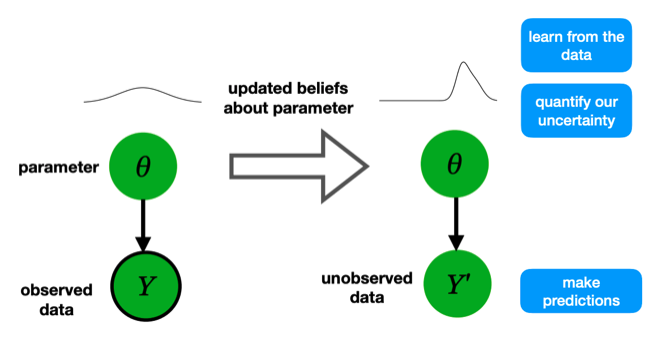
\includegraphics[width=\textwidth]{Bayesian_inference.png}
\end{figure}
	
	\begin{equation*}
		\pi\left(\theta \mid Y \right)=\frac{P(Y \mid \theta) \pi_0(\theta)}{Z}
	\end{equation*}
	
%	\begin{itemize}
%		\item We want to learn about $\pi$, typically by calculating expectations
%		$$\EE\{f(\Xt{})\} \defined \pi(f) \defined \int f(\xvec) \pi(\dx).$$ \pause
%		\item However, in general, the expectations can’t be done exactly. \pause
%		\item Approximate inference: Markov chain Monte Carlo (MCMC) constructs a Markov chain $\Yn{0}, \Yn{1}, \Yn{2}, \dots,$ such that $\Yndist{n} \to \pi$
%		\[
%		\sum_{n=1}^{N} f(\Yn{n}) / N \convas \pi(f) \quad\text{for } N \to \infty. \label{eq:SLLN}
%		\]
%	\end{itemize}
\end{frame}

\begin{frame}{Bayesian Approximation}
%	\begin{figure}
%		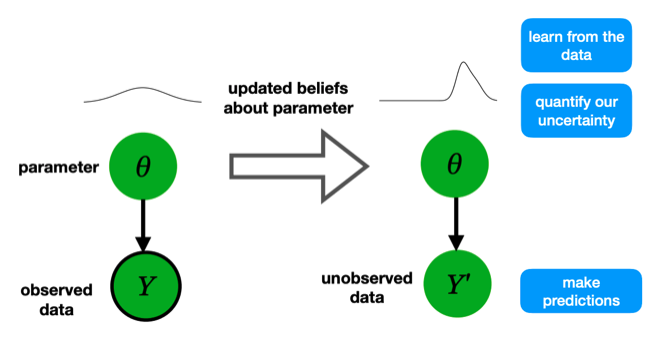
\includegraphics[width=\textwidth]{Bayesian_inference.png}
%	\end{figure}
	
	\begin{equation*}
		\pi\left(\theta \mid Y \right)=\frac{P(Y \mid \theta) \pi_0(\theta)}{Z}
	\end{equation*}
	
		\begin{itemize}
				\item We want to learn about $\pi$, typically by calculating expectations
				\begin{itemize}
					\item Find the mean and covariance of $\theta$ \pause
				\end{itemize}
%				$$\EE\{f(\Xt{})\} \defined \pi(f) \defined \int f(\xvec) \pi(\dx).$$ \pause
				\item However, in general, the expectations can’t be done exactly \pause
				\item Approximate inference: 
				\begin{itemize}
				\item Markov chain Monte Carlo (MCMC) 
				\end{itemize}
%				constructs a Markov chain $\Yn{0}, \Yn{1}, \Yn{2}, \dots,$ such that $\Yndist{n} \to \pi$
%				\[
%				\sum_{n=1}^{N} f(\Yn{n}) / N \convas \pi(f) \quad\text{for } N \to \infty. \label{eq:SLLN}
%				\]
			\end{itemize}
\end{frame}



\begin{frame}{Challenges in Modern Approximate Bayesian Inference}
	\begin{itemize}
		\item \textbf{Challenges:}
		\begin{itemize}
			\item high-dimensional $\theta \in \reals^{D}$, $D$ is large
			\item complex relationship $p(Y|\theta)$
			\item large-scale dataset
		\end{itemize}\pause
		\item \textbf{Problems of MCMC:}
		\begin{itemize}
			\item Slow convergence and poor mixing in complex cases e.g. those involving heterogeneity or high correlation between coordinates
			\item Computational cost of likelihood evaluation is proportional to the dataset size
%			\item Diagnosing convergence is harder in high dimensions.
		\end{itemize} \pause
		\item \textbf{Mitigations:}
		\begin{itemize}
			\item Variational Inference (VI).
			\item Subsampling methods (e.g. Stochastic Gradient Langevin Dynamics (SGLD)).
		\end{itemize}
	\end{itemize}
\end{frame}

%\begin{frame}{Overview}
%	\begin{itemize}
%		\item A priori finite-time, finite-data guarantees:\\
%		A Unifying Framework for Understanding General-purpose Bayesian Posterior Approximation Methods, \\
%		Huggins, Kasprzak, \textbf{Wang}, Campbell, Broderick. In prep
%		\item A post hoc quality check for VI: \\A Targeted Accuracy Diagnostic for Variational Approximations (TADDAA), \textbf{Wang}, Kasprzak, Huggins. AISTATS 2023.
%		\item Uncertainty quantification for Subsampling methods:\\
%		Stationary Analysis of Fixed Learning Rate Stochastic Gradient Algorithms, \textbf{Wang} $\&$ Huggins. (Under Review)
%	\end{itemize}
%\end{frame}

\begin{frame}{Overview}
	\begin{itemize}
		\item \textcolor{gray}{A priori finite-time, finite-data guarantees:\\
		A Unifying Framework for Understanding General-purpose Bayesian Posterior Approximation Methods, \\
		Huggins, Kasprzak, \textbf{Wang}, Campbell, Broderick. In prep} \pause
		\item \textbf{A post hoc quality check for VI}: \\A Targeted Accuracy Diagnostic for Variational Approximations (TADDAA), 
		
		\textbf{Wang}, Kasprzak, Huggins. AISTATS 2023.
		\item \textbf{Uncertainty quantification for Subsampling methods}:\\
		Stationary Analysis of Fixed Learning Rate Stochastic Gradient Algorithms, 
		
		\textbf{Wang} $\&$ Huggins. (Under Review)
	\end{itemize}
\end{frame}

% Section 1
\section{TADDAA}

\begin{frame}
  \frametitle{Markov chain Monte Carlo (MCMC) }
%  MCMC sampling methods provide a general-purpose framework for obtaining samples that are asymptotically exact.
  \begin{itemize}
  \item \textbf{Proposal distribution:} $\proposal{\state}{\proposedState}{\proposalParam}$ parameterized by $\proposalParam$ with current state $\state$ and corresponding density $\proposalDensity{\state}{\proposedState}{\proposalParam}$.
  \item \textbf{Metropolis--Hastings (MH) correction:} to construct a Markov kernel with the desired stationary distribution $\pi$, a proposed state 
$\mcProposedState \distas Q_{\psi}(x, \cdot)$ 
is accepted with probability 
\[ \label{eq:MH-accept}
\acceptprob{\state}{\mcProposedState} 
= \min \left\{1, \frac{\posteriorDensity(\mcProposedState) \proposalDensity{\mcProposedState}{\state}{\proposalParam}}{\posteriorDensity(\state) \proposalDensity{\state}{\mcProposedState}{\proposalParam}}\right\}. 
\]
  \end{itemize}
\end{frame}

\begin{frame}{Variational Inference (VI)}
Variational inference (VI) provides a potentially faster alternative to MCMC when models are complex and/or the dataset size is large.
\[
\hat{\posteriorDensity}   = \argmin_{\xi \in \mathcal{Q}} \mathcal{D}_{\posteriorDensity}(\xi).
\]
\begin{itemize}
%     \item VI aims to minimize some measure of discrepancy $\mathcal{D}_{\mainmeas}(\cdot)$ in a tractable family $\mathcal{Q}$ of potential
% approximating distributions
% \[ \hat{\mainmeas}   = \argmin_{\xi \in \mathcal{Q}} \mathcal{D}_{\mainmeas}(\xi). \]
    \item Variational family $\mathcal{Q}$: we are able to efficiently calculate
expectations of interest (e.g. mean and variance).  
    \item Measure of discrepancy $\mathcal{D}_{\pi}(\cdot)$: the canonical choice is \emph{Kullback--Leibler (KL) divergence} out of convenience. 
%\[
%\mathcal{D}_{\posteriorDensity}(\xi) = \mathrm{KL}(\xi \mid \posteriorDensity) :=\int \log \left(\frac{\mathrm{d} \xi}{\mathrm{d} \posteriorDensity}\right) \mathrm{d} \xi.
%\]
\end{itemize}
\end{frame}

\begin{frame}{Related Works}
\begin{itemize}
    \item Existing evaluation tools:
    \begin{itemize}
        \item Evidence Lower Bound (ELBO)
        \item Kernel Stein Discrepancy (KSD)\footnote{Gorham et al. (2017). Measuring sample quality with kernels.International Conference on Machine Learning.}
        \item Pareto smoothed importance sampling (PSIS) $\hat{k}$\footnote{Yao et al. (2018) Yes, but did it work?: Evaluating variational inference. 35th International Conference on Machine Learning (ICML).}
        \item $W_{2}$ upper bound\footnote{Huggins et al. (2020) Validated variational inference via practical posterior error bounds. AISTATS}
    \end{itemize}
    \item Problems:
    \begin{itemize}
        \item Lack interpretability
        \item Not applicable in high-dimensional parameter spaces.
        \item Don't support marginal checks
    \end{itemize}
\end{itemize}
\end{frame}

\begin{frame}{TADDAA: Intuition}
	
  We want to quantify approximation error $\varepsilon^{(0)} \defas \mu(\initialDensity) - \textcolor{red}{\mu(\posteriorDensity)}$ 
%  for a posterior functional of interest $\mcF$ such as a mean or variance.
  \begin{columns}
    \begin{column}{.44\textwidth}
      \begin{figure}[t]
        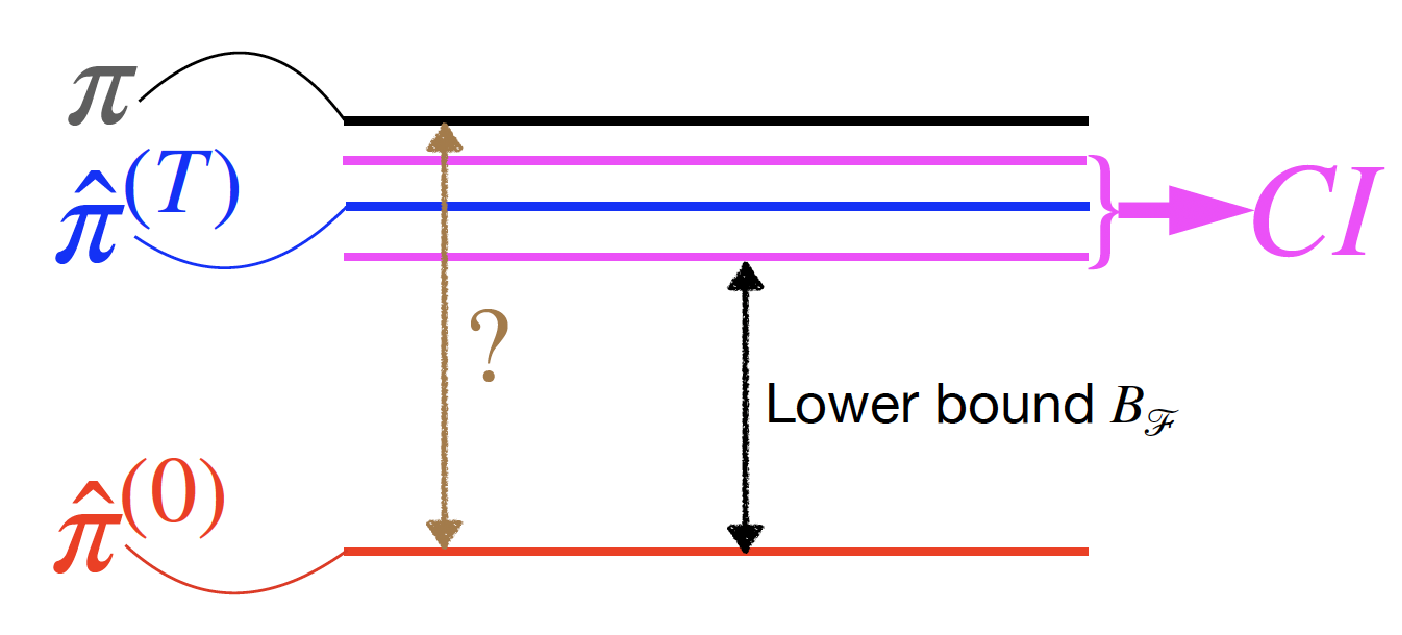
\includegraphics[width=\textwidth]{intuition_plot.pdf}
        \caption{$\hat{\pi}^{(T)}$ significantly different from $\hat{\pi}^{(0)}$ $\Rightarrow$ $\hat{\pi}^{(0)}$ far from $\pi$.}
      \end{figure}
    \end{column}
    \begin{column}{.6\textwidth}
        \begin{itemize}
        \item For another approximation $\hat{\pi}^{(T)}$ closer to taget posteriror $\pi$, $\varepsilon^{(T)} \defas \mu(\improvedDensity) - \textcolor{red}{\mu(\posteriorDensity)}$
        \item 
        \begin{equation*}
		\begin{aligned}
			&\varepsilon^{(0)}
			\ge |\mu(\initialDensity) - \mu(\improvedDensity)| \\
%			&\ge \begin{cases}
%				0 & \text{if $\ell_{\mu} \le 0 \le u_{\mu}$} \\
%				\min(|\ell_{\mu}|, |u_{\mu}|) & \text{otherwise} 
%			\end{cases} \\
%			&= \mathbf{1} \left\{0 \notin (\ell_{\mu},  u_{\mu})\right\} \times \min(|\ell_{\mu}|, |u_{\mu}|) \\
%			&\defines  B_{\mu}. 
		\end{aligned}
		\end{equation*}
        \end{itemize}
    \end{column}
  \end{columns}
  
\end{frame}

\begin{frame}{Example: Low-quality VI}
  \begin{columns}
	\begin{column}{.44\textwidth}
		\begin{figure}[t]
			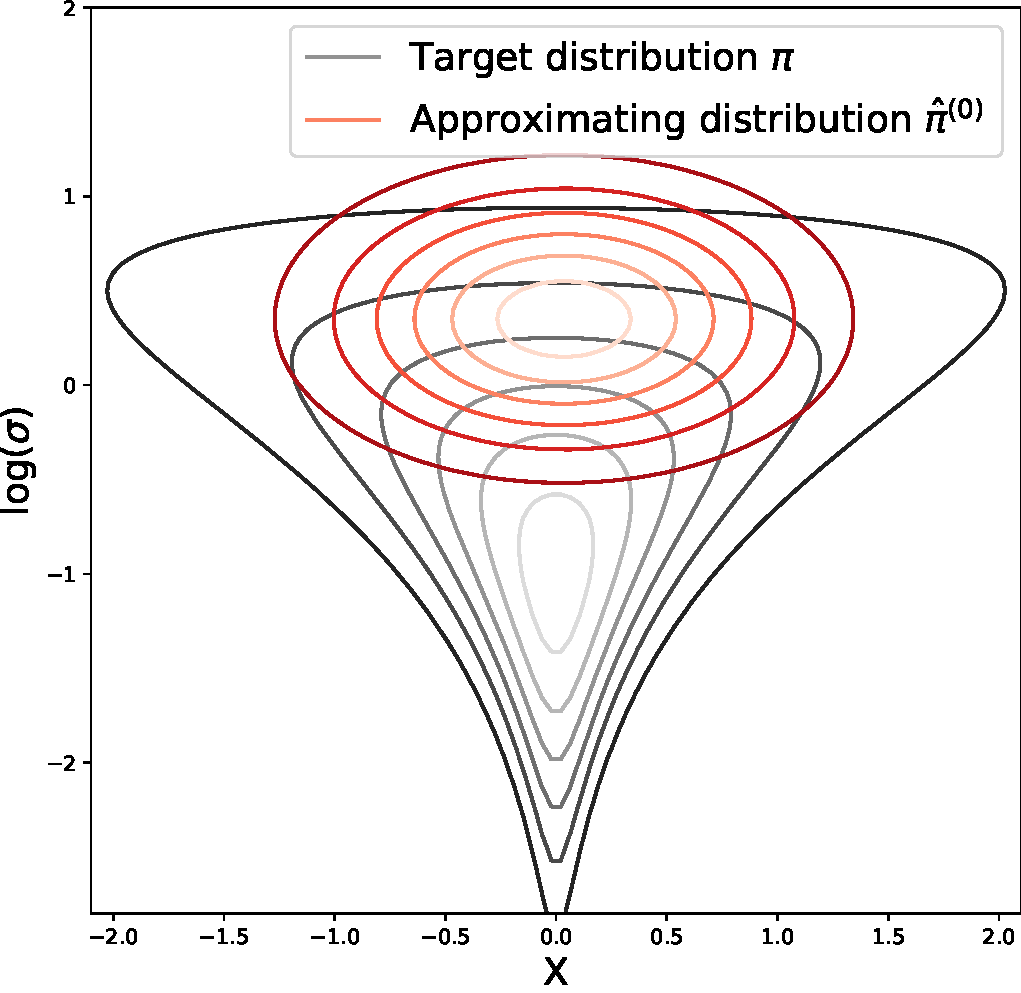
\includegraphics[width=\textwidth]{neal_vi.pdf}
			\caption{Variational approximation on 2-D Neal-Funnel shape model.}
		\end{figure}
	\end{column}
	\begin{column}{.6\textwidth}
%Neal's example has support for $\log(\sigma) \in \mathbb{R}$ and $x \in \mathbb{R}^{d-1}$. 
The parameterization of Neal-Funnel shape model is given as follows:
$$
\log(\sigma) \sim \mathcal{N}(0, \sigma_{0}^{2}), \quad x_{i} \sim \mathcal{N}(0,\sigma).
$$
%For illustrative purpose, let $\beta_{1}=\log(\sigma)$ and $\beta_{2}=x_{1}$.
	\end{column}
\end{columns}
\end{frame}

\begin{frame}{TADDAA Framework}
\begin{figure}[t]
	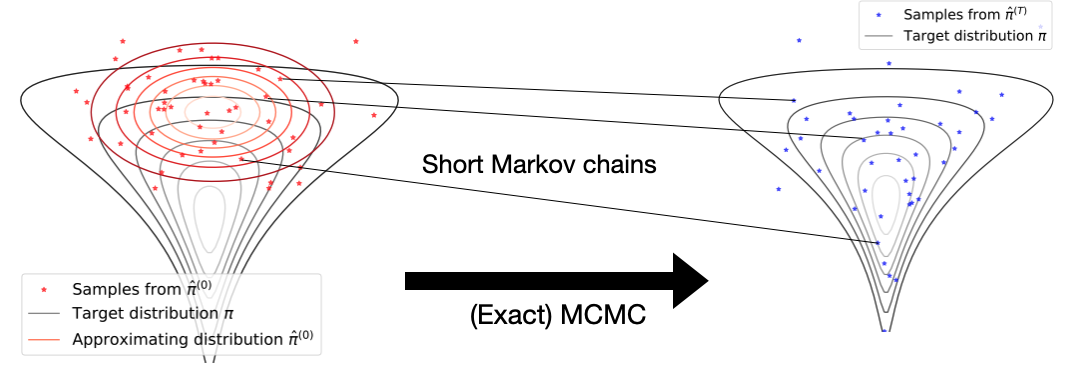
\includegraphics[width=\textwidth]{TADDAA_framework.png}
%	\caption{Variational approximation on 2-D Neal-Funnel shape model.}
\end{figure} \pause

\textcolor{red}{\textbf{Why not use MCMC directly?}}
\begin{itemize}
	\item Slow convergence in complicated cases.
	\item TADDAA \textbf{DOES NOT} rely on convergence of Markov chains.
\end{itemize}

\end{frame}


\begin{frame}{TADDAA:Input}
\begin{columns}
  \begin{column}{0.5\linewidth}
\begin{figure}
  \begin{center}
    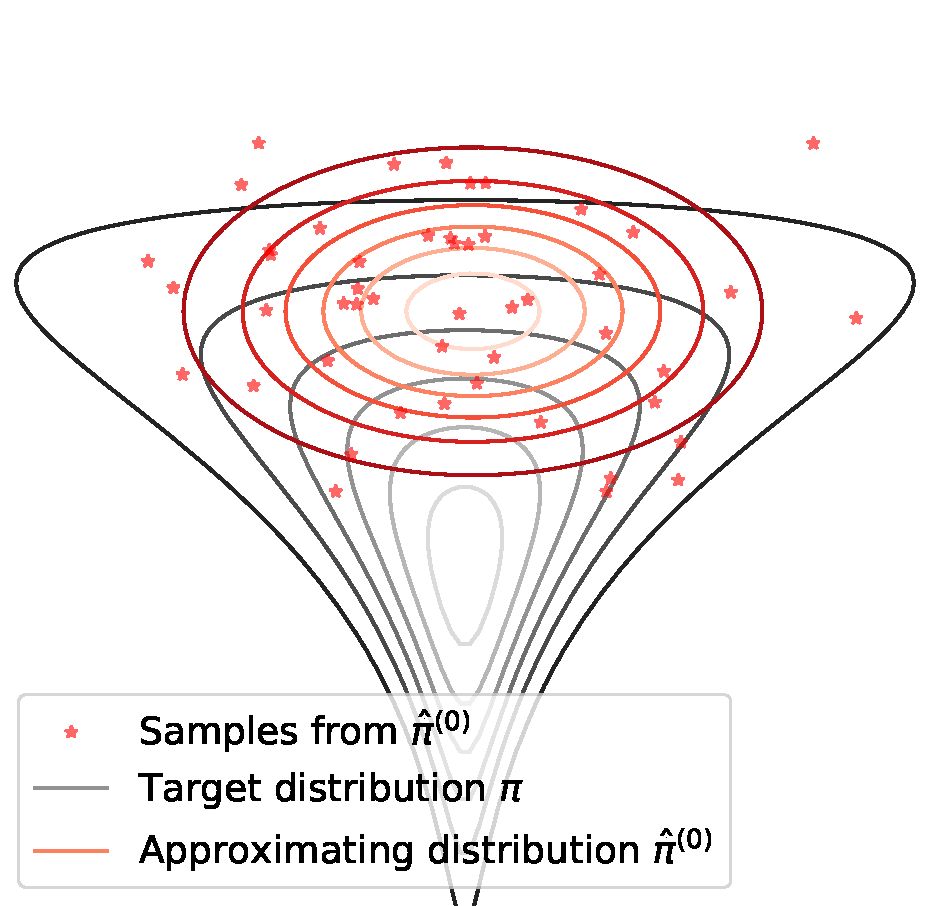
\includegraphics[width = \textwidth]{neal_vi_sample.pdf}
  \end{center}
\end{figure}
  \end{column}
  \begin{column}{0.5 \linewidth}

       %\textbf{\textcolor{blue}{1.Input:}}
       % \heading{\textcolor{blue}{Input:}}
        \begin{itemize}
            \item log density of the target $\pi$
            \item approximating distribution $\hat{\pi}^{(0)}$ \pause
            \item functional of interest $\mathcal{F}$ (e.g. marginal mean) \pause
            \item transition kernel $K_h(x, \mathrm{~d} y)$ (e.g. Barker, HMC) %and $\psi^{(0)}$
            \item number of Markov chains $N$ and iterations $T$
        \end{itemize}
  \end{column}
\end{columns}
\end{frame}

\begin{frame}{TADDAA:Run MCMC with inter-chain adaptation (INCA)}
  \begin{columns}
  \begin{column}{0.5\linewidth}
\begin{figure}
  \begin{center}
    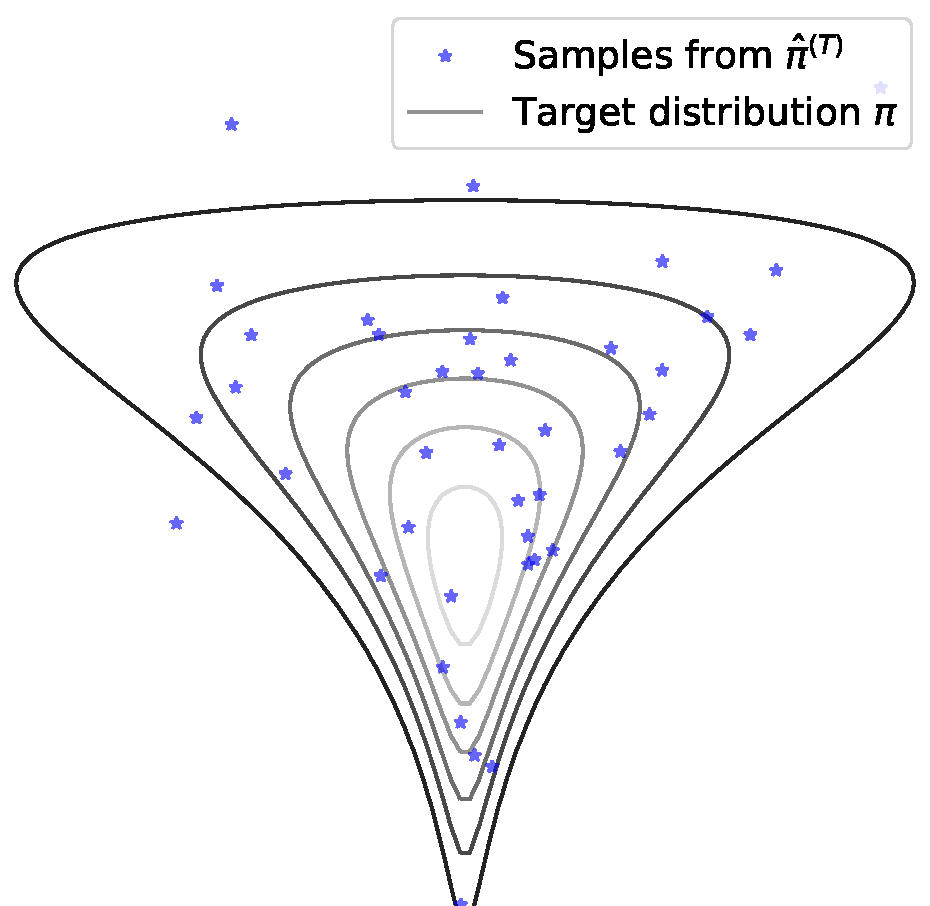
\includegraphics[width = \textwidth]{neal_vi_improved_samples.pdf}
  \end{center}
\end{figure}
  \end{column}
  \begin{column}{0.6 \linewidth}
        %\textbf{\textcolor{blue}{2.Run MCMC with inter-chain adaptation:}}
        % \heading{\textcolor{blue}{2.Run MCMC with inter-chain adaptation (INCA):}} %use for loop
        % \begin{itemize}
        %     \item $X_{j}^{(t+1)} \sim K_{\psi^{(t)}}\left(X_{j}^{(t)}, \cdot\right)$
        %     \item $\psi^{(t+1)}=H\left(\psi^{(1: t)}, X_{1: N}^{(1: t+1)}, Y_{1: N}^{(1: t+1)}\right)$
        % \end{itemize}
        \textbf{\quad for} $t=0$ to $T-1$ \textbf{do}:\\
        \textbf{\quad\qquad for} $j=1$ to $N$ \textbf{do}:
        \text{\qquad\qquad $X_j^{(t+1)} \sim K_{h^{(t)}}(X_j^{(t)}, \cdot)$}\\
            % & \qquad\qquad \alpha_j^{(t)}=\alpha(X_j^{(t)}, Y_j^{(t)}) \\
            % & \qquad\qquad X_j^{(t+1)}= \begin{cases}Y_j^{(t)}, & \text { with probability } \alpha_j^{(t)} \\
            % X_j^{(t)}, & \text { with probability } 1-\alpha_j^{(t)}\end{cases}
            % & \qquad\qquad \text{accept} $ Y_j^{(t+1)}$ with probability $\alpha_j^{(t)}$
        \textbf{\quad\qquad end for}\\
        \text{\quad\qquad update step-size $h^{(t+1)}$ using INCA.}\\
        \text{\quad\textbf{end for}}
  \end{column}
  \end{columns}
\end{frame}

\begin{frame}{TADDAA:Compute error lower bounds}
\begin{columns}[T]
  \begin{column}{0.5\linewidth}
\begin{figure}[p]
    \centering 
    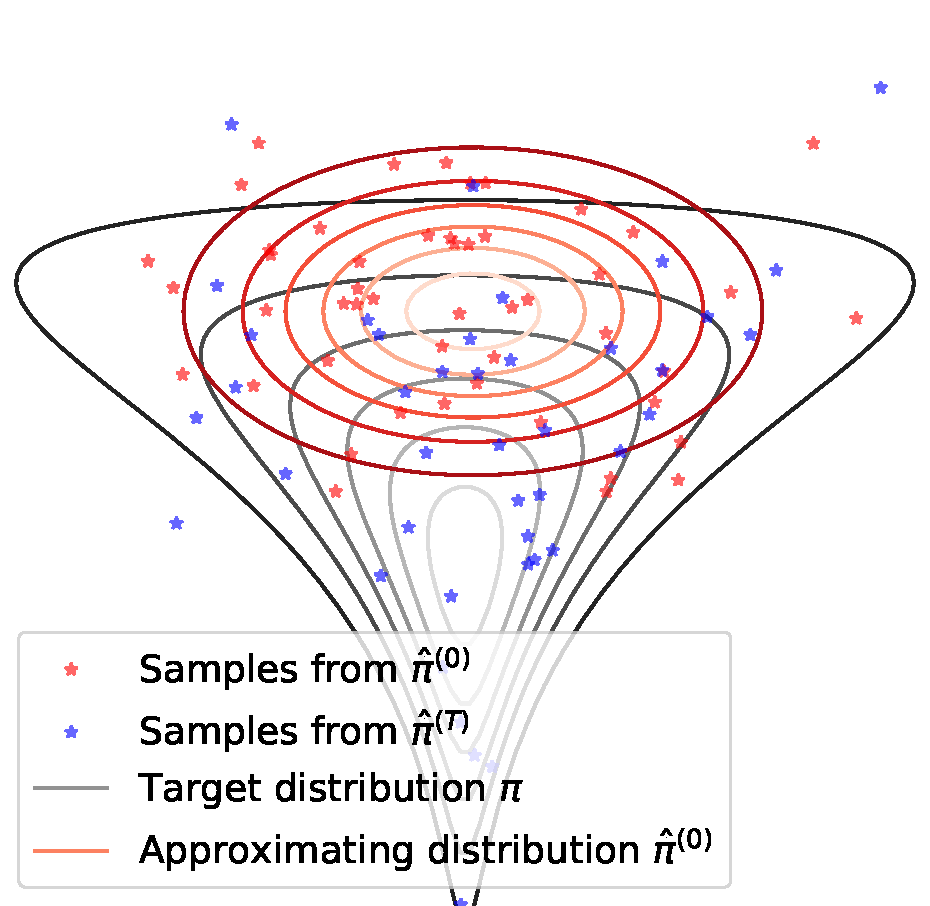
\includegraphics[width = \textwidth]{neal_vi_all_samples.pdf}
\end{figure}
  \end{column}
  \begin{column}{0.5 \linewidth}
        %\textbf{\textcolor{blue}{3.Compute error lower bounds and reliability check:}}
        % \heading{\textcolor{blue}{3.Compute error lower bounds and reliability check:}}
        \begin{itemize}
%                \item Compute correlation check $\rho_{\max }^2(T)$
                \item Compute a confidence interval $(\ell_{\mathcal{F}}, u_{\mathcal{F}})$ for $\mathcal{F}(\hat{\pi}^{(0)})-\mathcal{F}(\hat{\pi}^{(T)})$ based on $X_{1: N}^{(0)}$ and $X_{1: N}^{(T)}$
                \item Compute lower bound $B_{\mathcal{F}}$
        \end{itemize}
  \end{column}
  \end{columns}
\end{frame}

% \begin{frame}{Functional of interest $\mathcal{F}$}
% % For $t \in \{0,\dots, T\}$, define the mean vector
% % $\mu^{(t)} = (\mu_{1}^{(t)}, \ldots, \mu_{d}^{(t)})^{\top} \defas  \EE_{X \sim \improvedDensityAt{t}}(X)$, 
% % %$\Sigma^{(t)} \defas \cov_{X \sim \improvedDensityAt{t}} (X)$,
% % and marginal standard deviations $\sigma^{(t)}_{i} \defas \operatorname{stdev}_{X \sim \improvedDensityAt{t}}(X_{i})$ for $i = 1,\dots,d$.
% \begin{itemize}
%     \item Marginal mean $\mcF_{\text{mean}}^{i}(\posteriorDensity) \defas \mu_{i}(\posteriorDensity) \defas \int x_{i}\,\posteriorDensity(\dee x)$
% \end{itemize}
% \end{frame}

\begin{frame}{Transition kernel $K_h(x, \mathrm{~d} y)$}
%Let $x \in \reals^{d}$ denote the current state, 
%$h \in \reals_{+}$ the step size, and $G \in \reals^{d \times d}$ a positive semi-definition preconditioning matrix. 
\begin{itemize}
    \item Random Walk Metropolis-Hasting (RWMH). 
    \item Metropolis-adjusted Langevin algorithm (MALA).
    \item Hamiltonian Monte Carlo (HMC).
    \item \textbf{Barker Proposal\footnote{Livingstone et al. The Barker proposal: combining robustness and efficiency in gradient-based MCMC. Journal of the Royal Statistical Society Series B: Statistical Methodology (2022)} (recommended choice)}
    \begin{itemize}
    	\item robust to precise step size and acceptance rate. 
    	\item high sampling efficiency.
    \end{itemize}
\end{itemize}
\end{frame}

\begin{frame}{Step size $h$}
%All four kernels rely on a step-size parameter $h^{(t)}$, to guarantee superior sampling efficiency when dimension $d$ is large, $h^{(t)}$ should be adapted according to \emph{inter-chain adaptation} (INCA) and \emph{optimal scaling}.
Step size adaption: 
            \begin{itemize}
                \item \textbf{Inter-chain adaptation(INCA)}\footnote{Craiu et al. Learn from thy neighbor: Parallel-chain and regional adaptive MCMC. Journal of the American Statistical Association (2009).}
                \begin{itemize}
                	\item $Y_{j}^{(t+1)} \distas Q_{h^{(t)}}(X_{j}^{(t)}, \cdot)$, accept with probability $\alpha^{(t)}_{j}$. 
                	\item $\bar\alpha^{(t)} = \frac{1}{N} \sum_{j=1}^{N} \alpha^{(t)}_{j}$.
                \end{itemize}
				\item \textbf{Optimal Scaling}\footnote{Roberts et al. Optimal scaling for various Metropolis-Hastings algorithms. Statistical science (2001).}
				
				\begin{itemize}
					\item  $
					\label{eq:adaptive step size}
					\log h^{(t+1)}= \log h^{(t)} +  \frac{1}{\sqrt{t+1}}(\bar\alpha^{(t)} - \bar{\alpha}_{*}),$
					$\bar{\alpha}_{*}$ is optimal asymptotic acceptance. 
				\end{itemize}
            \end{itemize} \pause
Optimal initial step size $h^{(0)}$ and $\bar{\alpha}_{*}$:
        \begin{itemize}
%            \item RWMH: $h^{(0)} = 2.4^2/d$, $\bar{\alpha}_{*} = 0.234$. 
            \item e.g. Barker: $h^{(0)} = {2.4^2}/{d^{1/3}}$, $\bar{\alpha}_{*} = 0.576$.
%            \item HMC: $h^{(0)} = {2.4^2}/{d^{1/4}}$, $\bar{\alpha}_{*} = 0.4$.
        \end{itemize} \pause 
\textcolor{red}{Problem:} INCA introduces dependence for $X_{1:N}^{(T)}$. 
\end{frame}

\begin{frame}{Asymptotic Independence of Adapted Markov Chains}
	$\CurrentSamples$ are dependent $\rightarrowtail$
	independence assumption of tests violated. \pause
	\begin{definition}
		Let $X_{N,1:N} = (X_{N,1}, \dots, X_{N,N})$ denote a random vector.
		The sequence of random vectors $\{ X_{N,1:N} \}_{N=1}^{\infty}$ is \textbf{$\bar\nu$-chaotic} if, 
		for any $r \in \nats$ and any bounded continuous real-valued functions $g_{1}, g_{2}, \ldots, g_{r}$,
		\[
		\begin{aligned}
			\lim _{N \rightarrow \infty}\EE_{X_{N,1:N}}\left\{\prod_{i=1}^{r}g_{i}\left(X_{N,i}\right)\right\}
			&= \prod_{i=1}^{r} \int g_{i}(x) \bar\nu(\dee x).
		\end{aligned}
		\]
		\label{chaos definition}
	\end{definition}
\end{frame}

\begin{frame}{Adapted Markov Chains are Chaotic}
	%\begin{assumption} 
	%	\label{assumption}
	%	%We have the following assumptions. 
	%	\begin{enumerate}
		%		\item \label{assumption1}%
		%		The proposal probability density $q_{h}(y, x)$ is continuous with respect to $(x, y, h)$.
		%		\item \label{assumption2}%
		%		The target distribution has a continuous probability density function $\posteriorDensity(\cdot)$.
		%		\item \label{assumption3}%
		%		Samples generated from the Markov transition kernel $T (x, y, h, \cdot, \cdot )$ satisfy $\EE \|X_{j}^{(t)}\|^{2} < \infty$ and $\EE \|Y_{j}^{(t)}\|^{2} < \infty$ for any $t \in \nats$.
		%	\end{enumerate}
	%\end{assumption}
	\begin{theorem}
		\label{propagation of chaos for x}
		Under some mild assumptions, for any $t \in \nats$, there exists a probability 
		distribution $\LimitingMeasureXt$ such that the sequence 
		$\{\CurrentSamples\}_{N=1}^{\infty}$ is $\LimitingMeasureXt$-chaotic.
	\end{theorem}
	
\end{frame}

\begin{frame}{Number of Markov chains $N$}
% The number of iterations has to be large enough that the improved distribution $\improvedDensity$ is sufficiently different from a poor approximating distribution $\initialDensity$.
%The number of Markov chains must be sufficiently large that the confidence intervals are small enough to detect meaningful errors.
%Hence, if the user's tolerance is $\delta_{\text{mean}}$ for relative mean error and $\delta_{\text{var}}$ for log variance error, then 
$N$ is determined by user's tolerance for statistical test error $\delta$, e.g.
\[
\begin{aligned}
	\label{eq:sample-size}
	\textstyle  N &= \textstyle  \max \left( N_{\text{mean}}, N_{\text{variance}}\right),
\end{aligned}
\]
where 
\[
\begin{aligned}
\textstyle N_{\text{mean}} &\defas \textstyle  \min \left\{ n \in \nats : \frac{t_{n-1}(\alpha / 2)}{\sqrt{n}} \leq \delta_{\text{mean}} \right\},  \\
\textstyle  N_{\text{variance}} &\defas  \textstyle  \min \left\{ n \in \nats :  \log\left( \frac{\chi^{2}_{n-1}(1-\alpha/2)}{\chi^{2}_{n-1}(\alpha/2)}\right) \leq \delta_{\text{var}} \right\}.
\end{aligned}
\]
\end{frame}

\begin{frame}{Number of iterations $T$}
Markov chain requires $\Theta(d^{\gamma})$ iterations to mix according to theory of optimal scaling \footnote{Roberts et al. Optimal scaling for various Metropolis-Hastings algorithms. Statistical science (2001).}. 
\begin{itemize}
    \item For RWMH, MALA, Barker: $T = \lfloor c d^{1/3} \rfloor$.
    \item For HMC: $T = \lfloor c d^{1/4}/L \rfloor, $
    where $L$ is the number of leapfrog steps in HMC. 
\end{itemize} \pause
\textbf{Remark}
\begin{itemize}
%    \item Based on our ablation studies, $c= 50$ is a reasonable choice. 
    \item Computational cost of TADDAA is comparable to VI:
    \begin{itemize}
        \item Computational cost for VI: $\Theta(d^{1/3})$\footnote{Bhatia, Kush, et al. Statistical and computational trade-offs in variational inference: A case study in inferential model selection.}.
        \item Computational cost for MALA and Barker: $\Theta(d^{1/3})$.
        \item Computational cost for HMC: $\Theta(d^{1/4})$.
    \end{itemize}
\end{itemize}
\end{frame}

\begin{frame}{A Reliability Check for the Diagnostic}
The reliability of TADDAA depends on the mixing behavior of the Markov chains: 

\begin{figure}[t]
	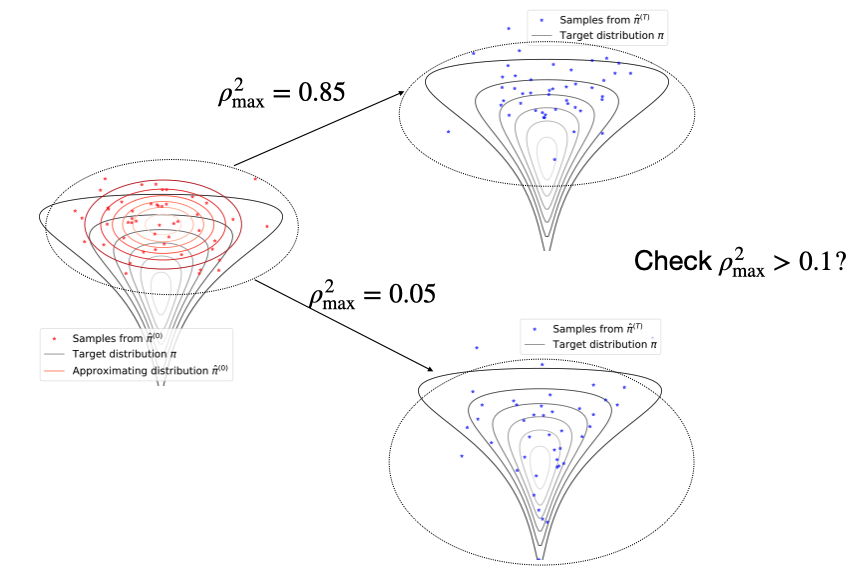
\includegraphics[width=\linewidth, height = 6cm]{reliability_check.png}
\end{figure}
%\begin{itemize}
%    \item Markov chains mixing well: TADDAA can be trusted.
%    \item Markov chains not mixing well:
%    \begin{itemize}
%    	\item Diagnosis of a poor approximation: TADDAA can be trusted.
%    	\item Diagnosis of a good approximation: \textbf{additional reliability check}.
%%    diagnosis of a poor approximation can still be trusted but diagnosis of a good approximation may not be reliable. \footnote{In the latter case, we should consider increasing the length of Markov chains or otherwise improving the Markov kernel.}
% 		\end{itemize}
% 		\pause
%		\item Reliability Check: 
%    \begin{itemize}
%    	\item Use worst-case correlation coefficient : $\rho^{2}_{\max}(T)
%    	\defas \max_{i} \rho^{2}_{i}(T)$.
%    	\item Check passes: $\rho^{2}_{\max}(T) < 0.1$.
%    \end{itemize}
%\end{itemize}

\end{frame}

%\begin{frame}{A Reliability Check for the Diagnostic (Continued)}
%% Instead, we propose to leverage the fact that we have many nearly independent chains to compute the correlation between the initial and final values of each chain.
%% If the chains are mixing, then this correlation will be close to zero. 
%% Specifically we propose to use the worst-case correlation coefficient
%
%\begin{itemize} 
%    \item We propose to use the worst-case correlation coefficient
%$
%\rho^{2}_{\max}(T)
%\defas \max_{i} \rho^{2}_{i}(T),
%%&= \max_{k}\frac{\sum_{j=1}^{N} ( X_{j,k}^{(0)}-\hat{\mu}_{k}^{(0)})( X_{j,k}^{(T)}-\hat{\mu}_{k}^{(T)})}{\sum_{j=1}^{N}( x_{j,k}^{(0)}-\hat{\mu}_{k}^{(0)})^{2} ( x_{j,k}^{(T)}-\hat{\mu}_{k}^{(T)})^{2}},
%$
%where 
%\[
%\begin{aligned}
%	% \rho^{2}\Big(X_{1:N,k}^{(0)},  X_{1:N,k}^{(T)}\Big)
%	\textstyle \rho^{2}_{i}(T)
%	\defas  \frac{\sum_{j=1}^{N} ( X_{j,i}^{(0)}-\hat{\mu}_{i}^{(0)})( X_{j,i}^{(T)}-\hat{\mu}_{i}^{(T)})}{\sqrt{\sum_{j=1}^{N}( X_{j,i}^{(0)}-\hat{\mu}_{i}^{(0)})^{2}} \sqrt{(\sum_{j=1}^{N} X_{j,i}^{(T)}-\hat{\mu}_{i}^{(T)})^{2}}}.
%\end{aligned}
%\]
%    \item Check passes: $\rho^{2}_{\max}(T) < 0.1$.
%    % \item $\rho^{2}_{\max}(T)$ large, then the check passes.
%\end{itemize}
%\end{frame}

%\begin{frame}{Revisit (High-dimensional) Neal-Funnel Shape Model}
%Neal's example has support for $\log(\sigma) \in \mathbb{R}$ and $x \in \mathbb{R}^{d-1}$. The parameterization of this model is given as follows:
%$$
%    \log(\sigma) \sim \mathcal{N}(0, \sigma_{0}^{2}), \quad x_{i} \sim \mathcal{N}(0,\sigma).
%$$
%For illustrative purpose, let $\beta_{1}=\log(\sigma)$ and $\beta_{2}=x_{1}$. In our experiment, $\sigma_{0}=1$.
%%\begin{figure}
%%    \centering 
%%    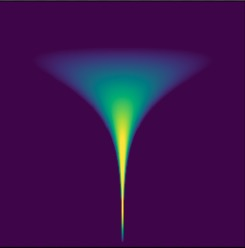
\includegraphics[width = 0.25\textwidth]{neal_funnel.jpg}
%%\end{figure}
%\end{frame}

\begin{frame}{Revisit (High-dimensional) Neal-Funnel Shape Model}
\begin{figure}[t]
    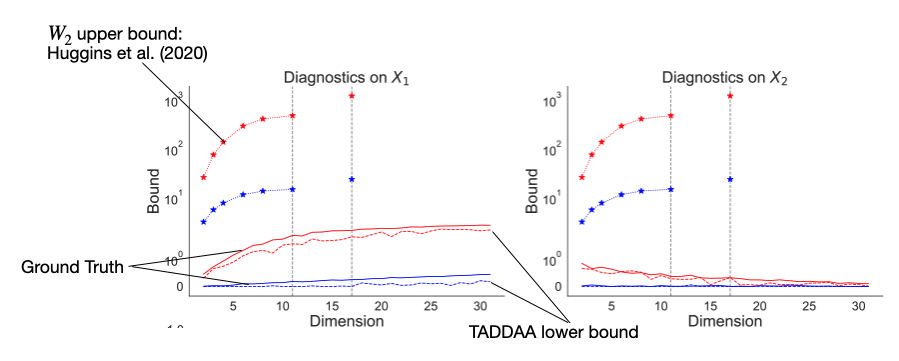
\includegraphics[width=\linewidth]{neal_high_new_1.png}
    \caption{Diagnostics for Neal-funnel shape model, where 
        %$B_{\text{mean}}$ and $B_{\text{variance}}$ are computed based on Barker proposal. 
        TADDAA uses the Barker proposal. 
        Here $\mu_{i}$ and $\sigma_{i}^{2}$ denote, respectively, the mean and variance of $X_{i}$. }
    \label{fig:High Dimensional Neal Funnel Diagnostics}
\end{figure}
\end{frame}

\begin{frame}{Revisit (High-dimensional) Neal-Funnel Shape Model}
	\begin{figure}[t]
		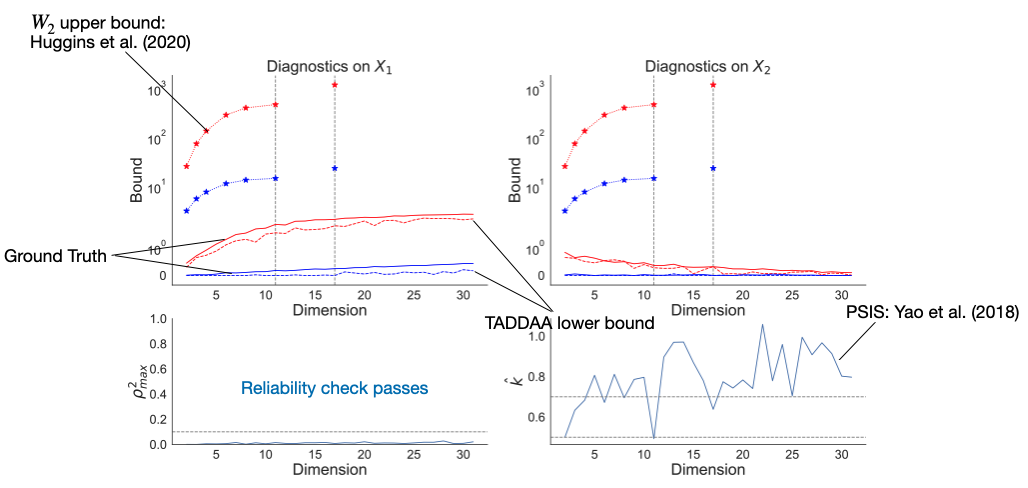
\includegraphics[width=\linewidth]{neal_high_new_2.png}
		\caption{Diagnostics for Neal-funnel shape model, where 
			%$B_{\text{mean}}$ and $B_{\text{variance}}$ are computed based on Barker proposal. 
			TADDAA uses the Barker proposal. 
			Here $\mu_{i}$ and $\sigma_{i}^{2}$ denote, respectively, the mean and variance of $X_{i}$. }
		\label{fig:High Dimensional Neal Funnel Diagnostics}
	\end{figure}
\end{frame}

\begin{frame}{Experiment: Neal-Funnel Shape Model}
Ablation study on $d=30$: the lower bounds become nearly constant at our proposed number of iterations $T$.
\begin{figure}
      \centering
      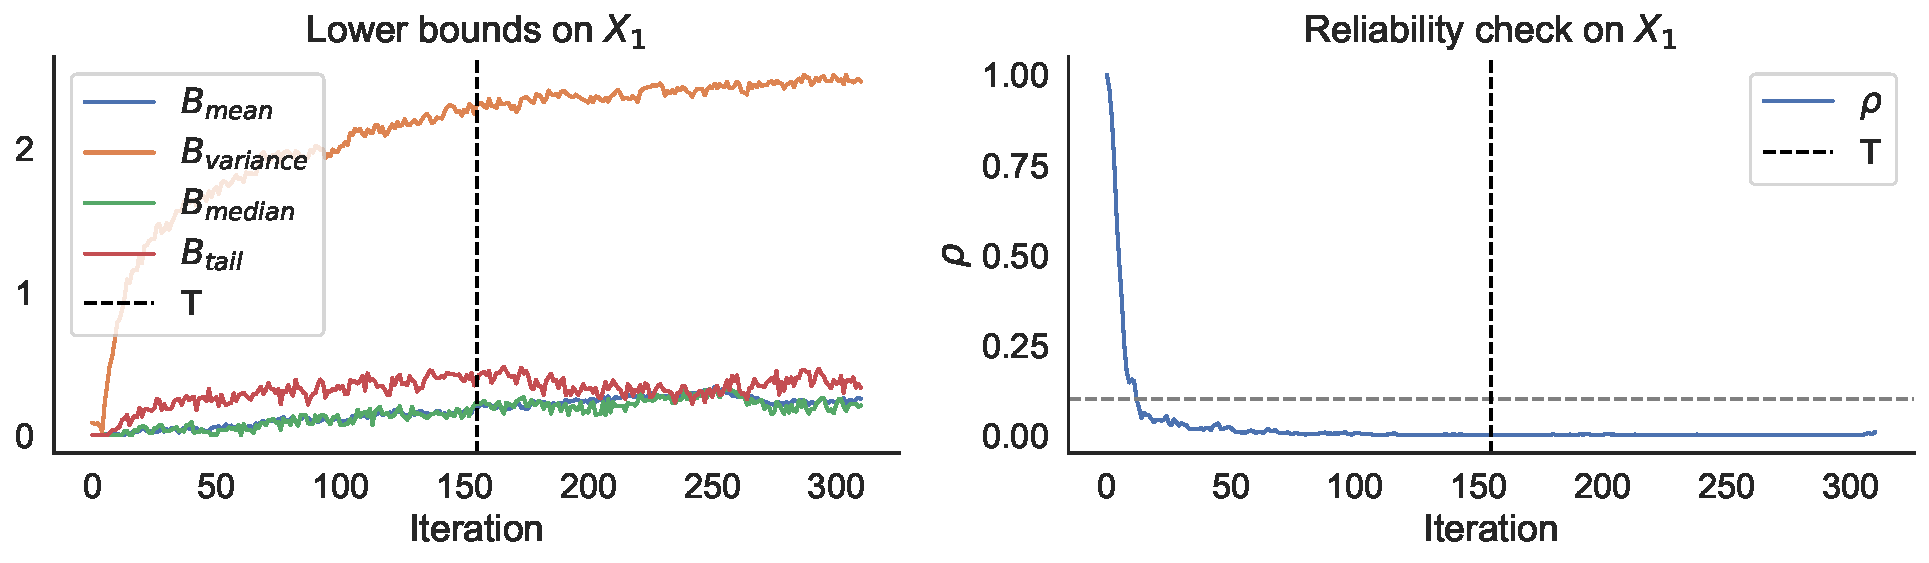
\includegraphics[width=\textwidth]{neal_high_iteration.pdf}
      %\caption{Another figure caption.}
\end{figure}
\end{frame}

\begin{frame}{Experiment: Logistic Regression Using Horseshoe Prior}
Use a logistic regression model with a sparsity-inducing horseshoe prior on 
\[
\begin{aligned}
    y &\mid \beta \sim \distBern(\operatorname{logit}^{-1}(X \beta)),\\
    \beta_{j} &\mid \tau, \lambda, c \sim \distNorm(0, \tau^{2} \tilde{\lambda}_{j}^{2}), \\
    \lambda_{j} &\sim \mathrm{C}^{+}(0,1), \qquad \tau \sim \mathrm{C}^{+}\left(0, \tau_{0}\right), \\
    c^{2} &\sim \distInvGam(2,8),
\end{aligned}
\]
where $y$ denotes the binary outcomes, $\tau >0 $ and $\lambda >0$ are global and local shrinkage parameters. 
\begin{itemize}
    \item $X \in \reals^{71 \times 100}$.
    \item Parameter dimension $d = 203$.
\end{itemize}
\end{frame}

\begin{frame}{Logistic Regression Using Horseshoe Prior: Mean Diagnostic}
\begin{itemize}
    \item Diagnostic:
    \begin{itemize}
    	\item capture both accurate and inaccurate marginal estimates
    	\item provide quite precise lower bounds
    \end{itemize}
    \item Computational efficiency: use $28\%$ as many gradient evaluations as VI.
\end{itemize}
     \begin{figure}
      \centering
      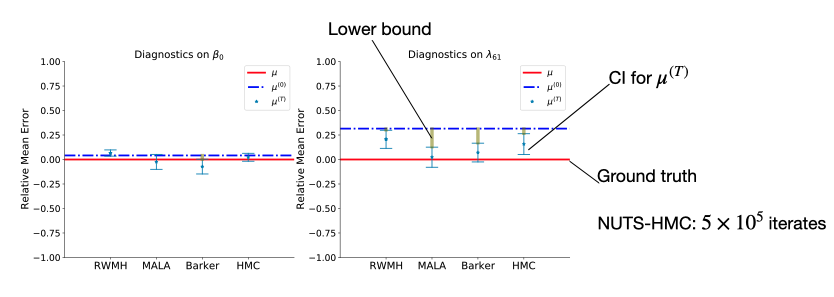
\includegraphics[width=\textwidth]{cancer_diagnostic_1.png}
      %\caption{Another figure caption.}
    \end{figure}
\end{frame}

\begin{frame}{Logistic Regression Using Horseshoe Prior: Variance Diagnostic}
	%	\begin{itemize}
		%		\item Diagnostic:
		%		\begin{itemize}
			%			\item capture both accurate and inaccurate marginal estimates
			%			\item provide quite precise lower bounds
			%		\end{itemize}
		%		\item Computational efficiency: use $28\%$ as many gradient evaluations as VI.
		%	\end{itemize}
	\begin{figure}
		\centering
		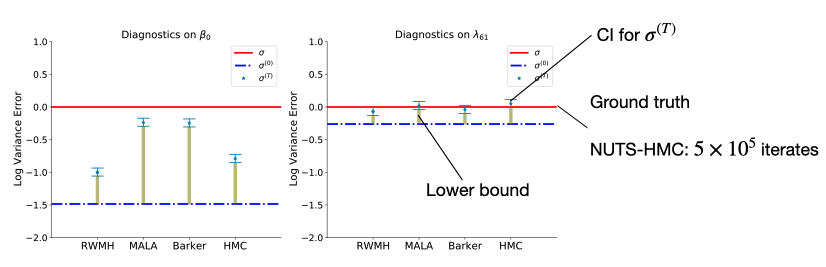
\includegraphics[width=\textwidth]{cancer_diagnostic_2.png}
		%\caption{Another figure caption.}
	\end{figure}
\end{frame}

\begin{frame}{Logistic Regression Using Horseshoe Prior: Reliability Check}
Reliability check: Barker and MALA pass reliability check, RWMH and HMC chains fail to mix. 
\begin{figure}
  \centering
  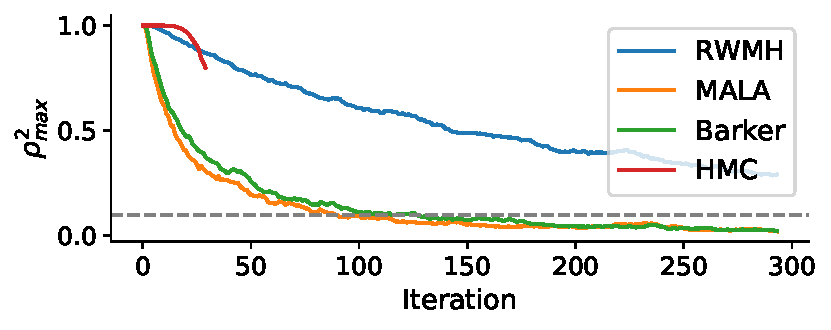
\includegraphics[width=0.8\textwidth]{cancer_reliability.pdf}
  %\caption{Another figure caption.}
\end{figure} 
\end{frame}

%\section{Conclusion}
\begin{frame}
	\frametitle{Conclusion}
	We propose a robust diagnostic tool for VI:
		\begin{itemize}
			\item supports marginal checks and is applicable to high-dimensional parameter spaces
			\item provides lower bounds on the error of specific posterior summaries
			\item is computationally efficient
			\item can be validated using a simple correlation-based reliability check
		\end{itemize}

\end{frame}


%\begin{frame}{Experiment: Logistic Regression Using Horseshoe Prior}
%	Reliability check: Barker and MALA pass reliability check, RWMH and HMC chains fail to mix. 
%	\begin{figure}
%		\centering
%		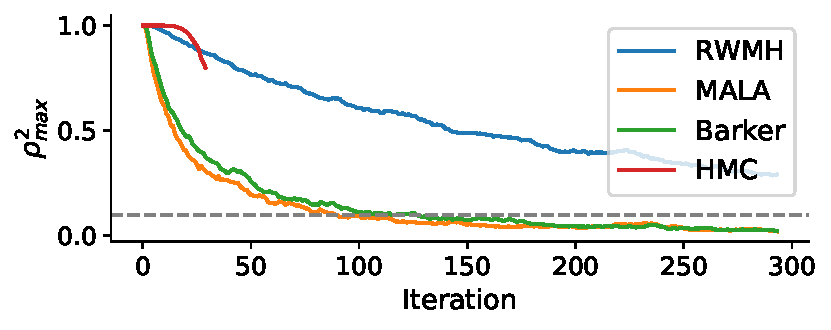
\includegraphics[width=0.8\textwidth]{cancer_reliability.pdf}
%		%\caption{Another figure caption.}
%	\end{figure} 
%\end{frame}


% Section 2
\section{Stationary Analysis of Fixed Learning Rate Stochastic Gradient Algorithms}
\begin{frame}{Stochastic optimization}
Consider data $\{x_{n}\}_{n=1}^{N}$ with $x_{n} \in \obsSpace$. 
For a parameter $\theta \in \reals^{D}$, observation-level differentiable loss 
$\ell : \obsSpace \times \reals^{D} \to \reals$, and regularizer $\reg : \reals^{D} \to \reals$, 
%bounded from below\fTBD{previously assumed non-negativity}, 
we aim to minimize the loss function
\begin{equation*}
\textstyle \loss(\theta) \defas N^{-1} \sum_{n=1}^{N} \ell(x_{n}, \theta) + N^{-1}\reg(\theta). 
\label{eq:loss function}
\end{equation*}\pause
\begin{itemize}
    \item Gradient Descnet (GD): $$\textstyle\theta_{t} = \theta_{t-1} - \Lambda \nabla \textstyle \loss(\theta_{t-1})$$\pause
    \item Stochastic Gradient Descnet (SGD): 
\begin{equation*}
\textstyle\theta_{t} = \theta_{t-1} - \Lambda G_{t}(\theta_{t-1}),
% -\Lambda B^{-1} \sum_{i \in S_{t}} \nabla \ell \left(x_{i}, y_{i}, \theta_{t-1} \right),
\label{eq: sgd update}
\end{equation*}
where $G_{t}(\theta) \defas B^{-1} \sum_{n \in S_{t}} \nabla \ell(x_{n}, \theta) + N^{-1} \nabla \reg(\theta)$ is the stochastic gradient.
    % with $\Lambda \in \reals^{D\times D}$ being a positive definite learning rate matrix.
\end{itemize}
\end{frame}

\begin{frame}{Subsampling Markov chain Monte Carlo (SGLD)}
SGLD is a Markov chain Monte Carlo (MCMC) algorithm equivalent to modifying SGD to include an additional Gaussian noise term
\begin{equation*}
\theta_{t} = \theta_{t-1} - \Lambda\,G_{t}(\theta_{t-1}) + \sqrt{2\beta^{-1} \Lambda}\,\xi_{t-1},
\label{eq: general SGLD update rule}
\end{equation*}
\begin{itemize}
    \item $\beta \in (0, \infty]$ is the inverse temperature (canonically set to $\beta = N$).
    \item $\xi_{t-1} \distiid \Norm(0, I)$.
\end{itemize}
\end{frame}

\begin{frame}{Goal}
We would like to accurately estimate the stationary covariance structure 
\begin{equation*}
\Sigma_{\theta} \defas \lim_{t \to \infty} \text{Cov} (\theta_{t}).
\end{equation*}

%Characterizing the stationary covariance can help quantify 
\begin{itemize}
	\item Accurately estimate the stationary covariance $\Sigma_{\theta}$ under fixed learning rates:
	\begin{itemize}
     \item Test loss
     \item Escaping efficiency from a sharp minimal\footnote{Zhu et al. (2019). The
     	anisotropic noise in stochastic gradient descent: Its behavior of escaping from sharp minima and regularization
     	effects. In International Conference on Machine Learning, pages 7654–7663. PMLR.}
     \end{itemize}
     \item Learning rate tuning guidance on optimal uncertainty quantification\footnote{Negrea et al. (2022). Tuning Stochastic Gradient Algorithms for Statistical Inference via Large-Sample Asymptotics.}
\end{itemize}
\end{frame}

\begin{frame}{Related Work: Quadratic Loss}
	Current works assume that the loss is well-approximated by a quadratic function\footnote{Mandt et al. (2017). Stochastic Gradient Descent as Approximate Bayesian Inference. Journal of Machine Learning Research.}:
	%\begin{condition}
	%	For all $t = 1,\dots,T$, it must hold that  
	\begin{equation*}
		\textstyle\loss(\theta_{t}) \approx \tilde{\loss}(\theta_{t}) := \frac{1}{2} \rbra[\big]{\theta_{t}-\MLEN}^{\top} \hess \rbra[\big]{\theta_{t}-\MLEN} + \mathrm{const},
		%\label{eq: approximate loss function}
	\end{equation*}
	where $\hess \defas \grad^{2} \loss(\MLE)$ is the Hessian of the loss (evaluated at $\MLE$). 
\end{frame}

\begin{frame}{Related Work: Continuous-time Proxies}
Approximate SGD by a continuous-time the Ornstein--Uhlenbeck (OU) process\footnote{Negrea et al. (2022). Tuning Stochastic Gradient Algorithms for Statistical Inference via Large-Sample Asymptotics.}
$$
	\dee \vartheta_{t} = -\Lambda \hess \vartheta_{t} \dee t + \Lambda \widehat{C}^{1/2} \dee W_{t},
$$
where $W_{t}$ be a $d$-dimensional Brownian motion and $\widehat{C} = \cov(G_{1}(\MLE))$ is the stationary gradient noise. \pause
\begin{itemize}
	\item The covariance matrix of the stationary distribution $\Sigma_{\vartheta} \defas \cov(\pi_{\vartheta})$ 
	satisfies 
	$$\Sigma_{\vartheta} \hess + \hess \Sigma_{\vartheta} = \Lambda \widehat{C}.$$ \pause
	\item \textcolor{red}{Limitation:} continuous-time proxies provide close approximation to SGD only for \textbf{small learning rates}.
\end{itemize}

\end{frame}

\begin{frame}{Related Work: Discrete-time proxies}
Under quadratic loss, the discrete-time proxy algorithm updates 
\begin{equation*}
	\label{eq:discrete-time-model-general}
	\psi_{t} = \psi_{t-1} - \frac{\Lambda}{B}\sum_{n\in S_{t}} \hess_{n} (\psi_{t-1} - \MLE),
\end{equation*}
where $\hess_{n} \defas  \grad^{2} \ell(x_{n}, \MLE)$.
\begin{itemize} \pause 
	\item \emph{Implicit} characterization of $\Sigma_{\psi}$\footnote{Liu et at. Noise and Fluctuation of Finite Learning Rate Stochastic Gradient Descent. ICML (2021).}:
	\begin{equation*}
		\Lambda \hess \textcolor{red}{\Sigma_{\psi}} + \textcolor{red}{\Sigma_{\psi}}  \hess \Lambda = \Lambda \left( \textcolor{blue}{\overline{C}_{\psi}}+ \hess \textcolor{red}{\Sigma_{\psi}} \hess \right)\Lambda,
		\label{eq: SGD stationary covariance}
	\end{equation*}
where $\textcolor{red}{\Sigma_{\psi}} \defas \cov(\pi_{\psi})$, and $\textcolor{blue}{\overline{C}_{\psi}} \defas \E[\cov\{G_{1}(\psi_{\infty})\}]$ is the expected covariance of the gradient noise. 
	\item For well-specified linear model and assume $X \sim \Norm(0, A)$\footnote{Liu et at. Strength of Minibatch Noise in SGD. ICLR (2022).}: 
	\begin{equation*}
		\textcolor{blue}{\overline{C}_{\psi}} %= \lim_{t \to \infty} \mathbb{E} \left[ C(\theta_{t})\right] 
		\approx B^{-1} \left( A \textcolor{red}{\Sigma_{\psi}} A + \Tr \left[ A \textcolor{red}{\Sigma_{\psi}} \right]A + \sigma^{2} A \right).
		\label{eq: sgd noise in well-specified linear model}
	\end{equation*}
	
\end{itemize}
	
\end{frame}

\begin{frame}{Limitations of discrete-time proxies}
	\textbf{Limitation: }
	\begin{itemize}
		\item Assumptions often do not hold in practice:
		\begin{itemize}
			\item Sample size $N \gg D$ and $N \to \infty$
			\item Mean Squared Error (MSE) loss
			\item The model is well-specified
		\end{itemize}
		\item There is no guarantee that the proxy process $(\psi_{t})_{t \ge 0}$ is close 
		to the original process $(\theta_{t})_{t \ge 0}$.
	\end{itemize} \pause
	
	\textbf{Contribution: }
	\begin{itemize}
	\item Propose a new discrete-time proxy algorithm that delivers more accurate stationary covariance estimates for: 
	\begin{itemize}
		\item Finite sample size $N$
		\item More general convex loss
		\item Misspecified model
	\end{itemize}
	\item Provide quantitative, non-asymptotic error analysis of our approximation.
\end{itemize}
\end{frame}

%\begin{frame}{Contributions}
%	\begin{itemize}
%		\item Propose a new discrete-time proxy algorithm that delivers more accurate stationary covariance estimates for: 
%		\begin{itemize}
%			\item Finite sample size $N$
%			\item More general convex loss
%			\item Misspecified model
%		\end{itemize}
%		\item Provide quantitative, non-asymptotic error analysis of our approximation.
%	\end{itemize}
%\end{frame}

\begin{frame}{A New Proxy Algorithm for Analyzing SG(L)D}
Our approach is to apply a second-order Taylor approximation to each loss term $\ell_{n}(\theta) \defas \ell(x_{n}, \theta)$:
\begin{equation*}
	\tilde\ell_{n}\left(\theta\right)  \defas \ell_{n}(\MLE) + \nabla \ell_{n}^{\top}( \MLE) (\theta-\MLE)+ (\theta-\MLE)^{\top}\grad^{2} \ell_{n}(\MLE) (\theta-\MLE).
	\label{eq: proxy algorithm framework for general loss}
\end{equation*}\pause

\begin{itemize}
	\item Minimizer $\MLE$ satisfies 
	$$
	\nabla\textstyle\loss(\MLE) = \frac{1}{N} N^{-1} \sum_{n =1}^{N} \nabla \ell(x_{n}, \MLE) + N^{-1} \nabla \reg(\MLE) = 0.
	$$
	\item In general, 
	$$
	B^{-1} \sum_{n \in S_{t}} \nabla \ell(x_{n}, \MLE) + N^{-1} \nabla \reg(\MLE) \neq 0.
	$$
\end{itemize}
\end{frame}

\begin{frame}{Stationary Fluctuation}
Our new proxy algorithm update:
\begin{equation*}
	\begin{aligned}
		\psi_{t} &= \psi_{t-1} -\frac{\Lambda}{B} \sum_{n \in S_{t}} \left\lbrace \nabla \ell_{n}\big(\MLE\big) +\mathcal{J}_{n} \big(\psi_{t-1}-\MLE\big)\right\rbrace \\
		&\quad - \frac{\Lambda}{N} \nabla \reg(\psi_{t-1}) + \sqrt{2\beta^{-1} \Lambda}\,\xi_{t-1}.
	\end{aligned}
	\label{eq: proxy discrete-time update for general loss}
\end{equation*}
	\begin{proposition} \label{thm:SGLD-stationary-covariance} 
		%\label{corollary: stationary covariance of SGLD}
		%Suppose the loss is well approximated by  a quadratic function \cref{eq: approximate loss function}, let $\theta_{t}$ be updated according to \cref{eq: general SGLD update rule}. 
		%The stationary noise is, for a fixed learning rate matrix $\Lambda$, the stationary covariance $\Sigma$ satisfies
		Assuming the iterates $(\psi_{t})_{t \ge 0}$ have a well-defined stationary distribution, the stationary covariance $\Sigma_{\psi}$ satisfies 
		\begin{equation*}
			\Lambda \hess \textcolor{red}{\Sigma_{\psi}} + \textcolor{red}{\Sigma_{\psi}}  \hess \Lambda = \Lambda \big( \textcolor{blue}{\overline{C}_{\psi}} + \hess \textcolor{red}{\Sigma_{\psi}} \hess \big)\Lambda + 2\beta^{-1}\Lambda.
			\label{eq: SGLD stationary covariance}
		\end{equation*}
%		In particular, if $\Sigma_{\psi}$ commutes with $\overline{C}_{\psi}$ and $\Lambda$, then
%		\begin{equation} 
%			\Sigma_{\psi} = \left(\Lambda\overline{C}_{\psi} \Lambda + 2\beta^{-1}\Lambda\right)\big(\Lambda \hess + \hess \Lambda - \Lambda \hess^{2} \Lambda\big)^{-1}.
%			\label{eq: stationary covariance of SGLD}
%		\end{equation}
%		Or, to obtain covariance $\Sigma_{\psi} = \Sigma$, if $\Lambda$ commutes with $\Sigma \hess$, then set 
%		\begin{equation}
%			\begin{aligned}
%				\Lambda &= \rbra{\hess\Sigma + \Sigma \hess - 2\beta^{-1}I_{D}} \big(\overline{C}_{\psi} +  \hess \Sigma\hess\big)^{-1}.
%			\end{aligned}
%			\label{eq: discrete quadratic learning rate}
%		\end{equation}
	\end{proposition}
	
\end{frame}

\begin{frame}{Stationary Gradient Noise}
	\begin{theorem} \label{theorem: general case covariance matrix of noise}
		For the proxy algorithm, if $\reg(\theta) = \frac{1}{2} \theta^{\top}\Gamma \theta^{\top}$ and the mini-batches
		are sampled with replacement, then 
		%the expected stochastic gradient covariance at stationarity satisfies\fTBD{I changed $\mathcal{J}$ to $\hess$}
		\begin{equation*}
			\label{eq: covariance of stationary noise}
			\begin{aligned}
				\textcolor{blue}{\overline{C}_{\psi}} =\frac{1}{B} \left( \mathcal{I} - \frac{1}{N^{2}} \Gamma \MLE \MLE^{\top} \Gamma^{\top} + \frac{1}{N} \sum_{n=1}^{N} \mathcal{J}_{n} \textcolor{red}{\Sigma_{\psi}} \mathcal{J}_{n} -  \mathcal{J} \textcolor{red}{\Sigma_{\psi}} \mathcal{J} \right),
			\end{aligned} 
		\end{equation*}
		where $\mathcal{I} \defas  \frac{1}{N} \sum_{n=1}^{N} \nabla\ell_{n}\bigl(\MLE\bigr) \nabla\ell_{n}\bigl(\MLE\bigr)^{\top}$, $\mathcal{J}_{n} = \nabla^{2}\ell_{n}\bigl(\MLE\bigr)$.
	\end{theorem}
\end{frame}

\begin{frame}{Wasserstein Distance}
How to assess the accuracy of our proxy algorithm? \textbf{Wasserstein Distance}
\begin{itemize}
\item \[
W_{2}(\pi, \tilde\pi) = \inf \E(\norm{\theta - \tilde\theta}^{2})^{1/2},
\]
where the infimum is over all joint distributions of $(\theta, \tilde\theta)$ such that $\theta \dist \pi$ and $\tilde\theta \dist \tilde\pi$. 
\item $W_{2}(\pi_{\theta}, \pi_{\psi}) \leq \veps$ implies that \footnote{Huggins et al. Validated variational inference via practical posterior error bounds. AISTATS (2020)}
\begin{equation*}
	\begin{aligned}
		&\label{eq:general-stdev-and-cov-error-bounds}
		|\sigma_{\theta,d} - \sigma_{\psi,d}| \leq \veps~(d = 1,\dots,D) \\
		&\norm{\Sigma_{\theta} - \Sigma_{\psi}} \le 2 \veps (\norm{\Sigma_{\theta}}^{1/2} \wedge \norm{\Sigma_{\psi}}^{1/2} + \veps).
	\end{aligned}
\end{equation*}
\end{itemize}
\end{frame}

\begin{frame}{Error Analysis}
%\begin{theorem} \label{thm:wasserstein-error-bound}
%	Under standard assumptions and $\Lambda = \lambda I_{D}$ for some $\lambda \in (0, 1/(2L))$,
%	then, letting $\beta \defas 1 - \lambda\mu \rbra*{1 - 2\lambda L}$, $\overline{M} \defas \{N^{-1} \sum_{n=1}^{N} M_{n}^{2}\}^{1/2}$,
%	and $C_{s} \defas  \E\rbra{\norm{\psi_{s} - \MLE}^{4}}$, for all $t = 1,2,\dots$,
%	\begin{equation*}
%	\label{eq:wasserstein-error-bound} 
%	\begin{aligned}
%\lefteqn{W_{2}^{2}(\pi_{\theta,t}, \pi_{\psi,t})} \\
%&\le \beta^{t}W_{2}^{2}(\theta_{0}, \psi_{0})  
%+ \lambda  \overline{M} \left\lbrace \frac{\lambda  \overline{M}}{2} + \frac{2}{\mu}\right\rbrace  \sum_{s=1}^{t}\beta^{t-s}C_{s-1}. \nonumber
%	\end{aligned}
%	\end{equation*}
%\end{theorem}
\begin{corollary} \label{cor:stationary-wasserstein-error-bound} 
	Under the same assumptions stated above and with $\beta = \infty$ (i.e., for the case of SGD), there exists $L>0$, if $\lambda < L/4$, then 
	there exists an explicit constant $A$ such that 
	\[
	W_{2}(\pi_{\theta}, \pi_{\psi}) \le A\frac{\lambda}{B}.
	\]
\end{corollary}
\end{frame}

\begin{frame}{Experiments: Linear Regression}
To validate our theory, we compare the predicted stationary covariance structure under the fixed learning rate obtained from other theory with others.
\begin{itemize}
	\item \emph{Simulated misspecified data.}:
	\begin{equation*}
		\label{eq: linear regression misspecified model}
		y_{n} \dist \Norm(x_{n}^{\top}\theta_{\star}, 1+\|x_{i}\|_{2}^{2}),
	\end{equation*}
	where $\theta_{\star} \dist \Norm(0, I_{D})$ is fixed and $x_{n} \distiid \Norm(0, I_{D})$.
	\item Real-world dataset: \emph{Boston housing data.}
\end{itemize}
\end{frame}

\begin{frame}{Experiments: Linear Regression}
\begin{figure}
	\centering
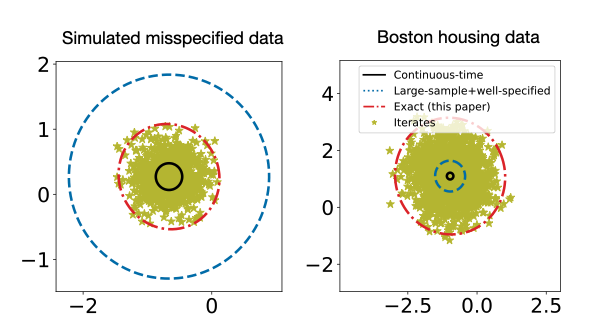
\includegraphics[width=\textwidth]{linear.png} 
\end{figure}
%\begin{figure}
%	\centering
%	\begin{minipage}[b]{0.4\textwidth}
%		\centering
%		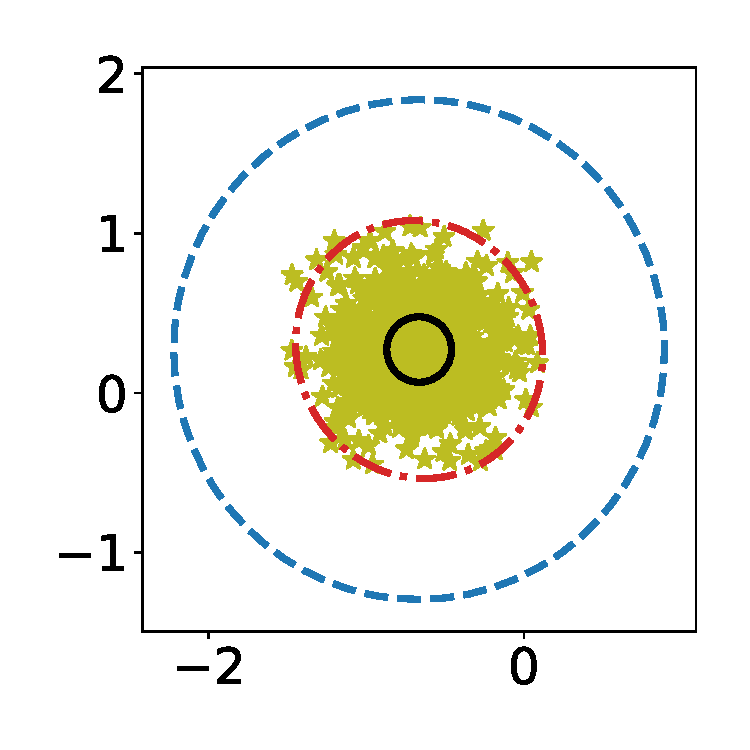
\includegraphics[width=\textwidth]{linear_simulation_single.pdf} 
%		%	\caption{First PDF}
%	\end{minipage}
%	\hspace{0.0001\textwidth}  % Space between the two PDFs
%	\begin{minipage}[b]{0.4\textwidth}
%		\centering
%		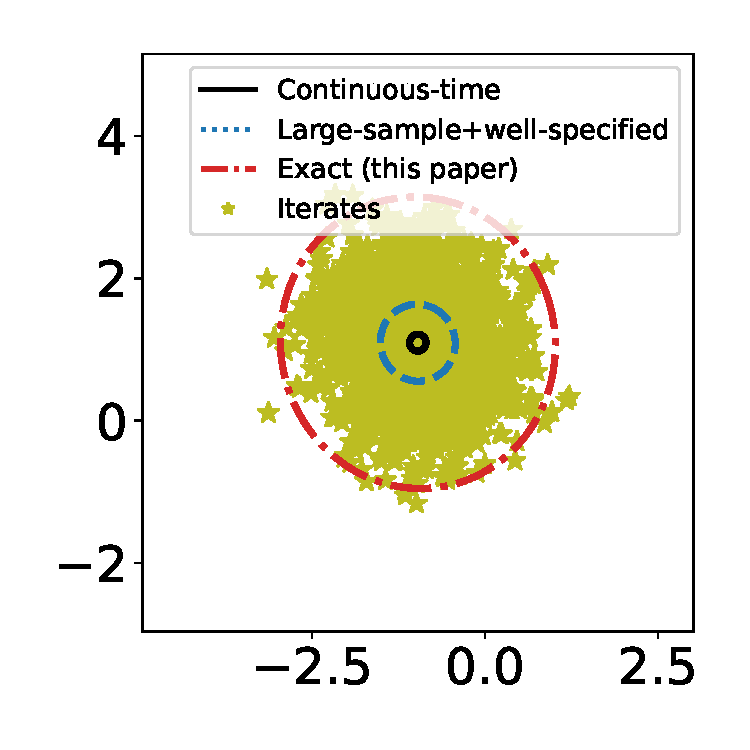
\includegraphics[width=\textwidth]{linear_real_single.pdf} 
%		%	\caption{First PDF}
%	\end{minipage}
%	%\caption{Compare learning rate tuning guidance suggested by different theories on a Boston Housing dataset.}
%%	\caption{Comparison of estimated stationary covariance structure for linear regression at $3\sigma$ confidence region on \textbf{(left)} simulated misspecified data with heteroskedastic noise 
%%		and \textbf{(right)} the classic Boston housing dataset with $\lambda = 0.1$ and $B = 32$.
%%		Our theory provides more accurate stationary covariance predictions in both cases.
%%	}\vspace{-1em}
%%	\label{Fig: linear regression fixed_lr}
%	%	\label{Fig: Linear regression on synthetic dataset_fixed_lr}
%\end{figure}
\end{frame}

\begin{frame}{Experiments: Poisson Regression}
\begin{itemize}
	\item \emph{Simulated well-specified data.}:
\begin{equation*}
	\label{eq: poission regression model}
	y_{n} \sim \text{Poisson}(\exp\{x_{n}^{\top}\theta_{\star}\}),
\end{equation*}
	where $\theta_{\star} \dist \Norm(0, I_{D})$ is fixed and $x_{n} \distiid \Norm(0, I_{D})$.
	\item Real-world dataset: \emph{German credit data.}
\end{itemize}
\end{frame}

\begin{frame}{Experiments: Poisson Regression}
	\begin{figure}
		\centering
		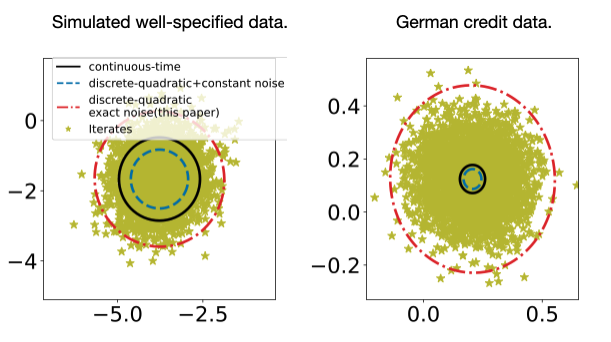
\includegraphics[width=\textwidth]{poisson.png} 
	\end{figure}
%\begin{figure}[t]
%	\centering
%	\begin{minipage}[b]{0.4\textwidth}
%		\centering
%		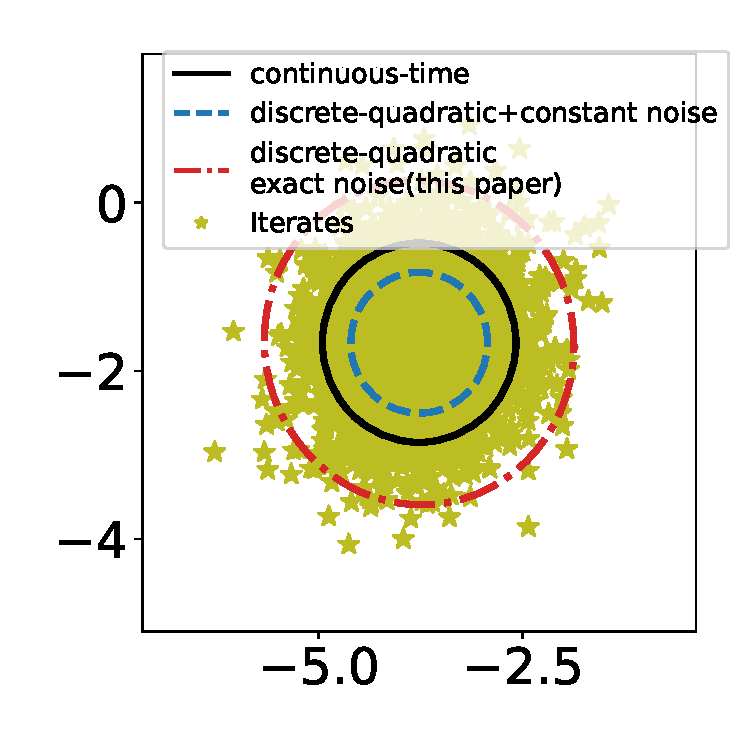
\includegraphics[width=\textwidth]{poisson_simulation_single.pdf} 
%		%	\caption{First PDF}
%	\end{minipage}
%	\hspace{0.0001\textwidth}  % Space between the two PDFs
%	\begin{minipage}[b]{0.4\textwidth}
%		\centering
%		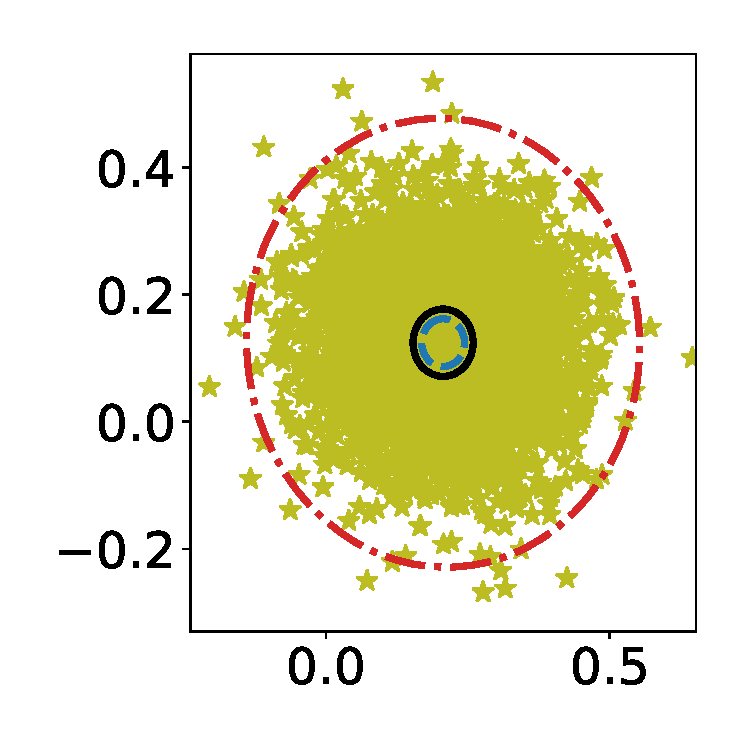
\includegraphics[width=\textwidth]{poisson_real_single.pdf} 
%		%	\caption{First PDF}
%	\end{minipage}
%	
%	\caption{Comparison of estimated stationary covariance structure for Poisson regression at $3\sigma$ confidence region with \textbf{(left)} simulated well-specified data and \textbf{(right)} the German credit data by setting batch size $\lambda = 0.1$, and $B = 32$.
%		%Our theory provides more accurate stationary covariance predictions in both cases.
%	} % synthetic and real-world dataset.}
%\label{Fig: Poisson regression fixed_lr}
%\end{figure}
\end{frame}




% Conclusion and Further work
%\section{Conclusion}

\begin{frame}
  \frametitle{Conclusion}
We have established a rigorous framework for understanding SGD and SGLD under:
\begin{itemize}
	\item  large learning rate. 
	\item $N$ is not large compared to $D$.
	\item model is incorrect.
\end{itemize}
\end{frame}

\section{Conclusion}

\begin{frame}{Conclusion}
	
\begin{enumerate}
	\item Post hoc quality check for variational approximation:
	\begin{itemize}
		\item support marginal checks
		\item robust in high-dimensional parameter sapce
		\item computationally efficient
	\end{itemize}
	\item Uncertainty quantification for subsampling methods: 
	\begin{itemize}
		\item Accurate stationary covariance structure estimation for stochastic gradient algorithms under fixed/nonvanishing learning rate
		\item Optimal learning rate tuning guidance 
	\end{itemize}
\end{enumerate}
	
\end{frame}


% A thank you slide
\begin{frame}{\Large Acknowledgments}
	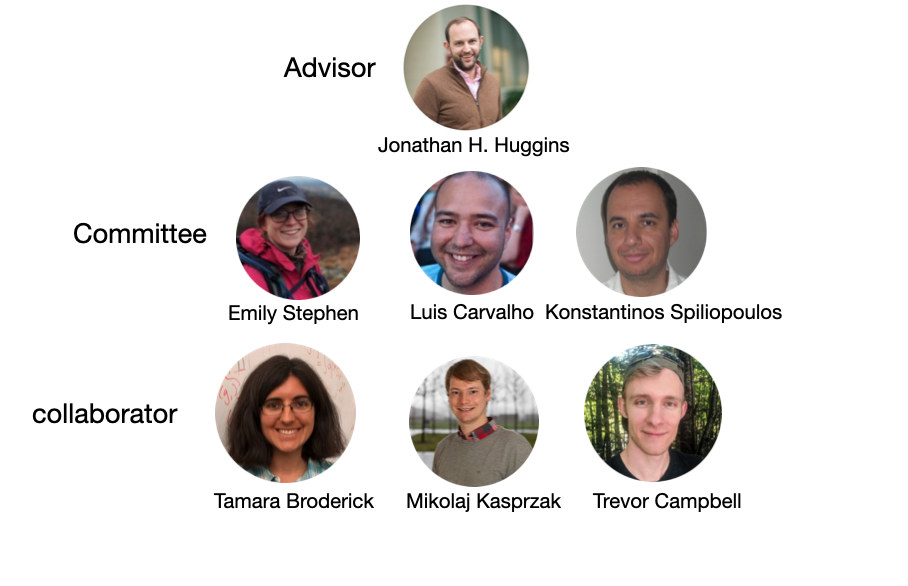
\includegraphics[width=\textwidth]{acknow.png} 
\end{frame}

\end{document}
